\chapter{Ecuaciones y sistemas}

\begin{tikzpicture}
	\fill [left color=red!50, right color=teal!50] (0,0) rectangle (6.5,.2);
	\fill [left color=teal!50, right color=blue!50] (6.5,0) rectangle (11.5,.2);
	\end{tikzpicture}


\vspace{10mm}
\begin{adjustwidth}{40pt}{40pt}
\begin{cuadro-gris}

	\begin{multicols}{2}
	$\triangleright \ $  Ecuaciones: 
	polinómicas, racionales, radicales, exponenciales, logarítmicas, con valor absoluto.
	
	$\triangleright \ $  Sistemas de ecuaciones: 
	lineales y no lineales
	\end{multicols}
\end{cuadro-gris}
\end{adjustwidth}


\vspace{1cm}
\section{Ecuaciones polinómicas}

\begin{tikzpicture}
	\fill [left color=red!50, right color=teal!50] (0,0) rectangle (3.5,.1);
	\fill [left color=teal!50, right color=blue!50] (3.5,0) rectangle (7.5,.1);
	\end{tikzpicture}
\vspace{0.5cm}


Una \textbf{ecuación} es una igualdad matemática entre dos expresiones, denominadas miembros y separadas por el signo igual, en las que aparecen elementos conocidos, \emph{datos}, y  desconocidos, \emph{incógnitas}, relacionados mediante operaciones matemáticas. No confundir con \emph{identidad}, una igualdad algebraica que es cierta para cualquier valor de la incógnita.

\subsection{Ecuaciones de primer grado}

\begin{tikzpicture}
	\fill [left color=red!50, right color=teal!50] (0,0) rectangle (3.5,.01);
	\fill [left color=teal!50, right color=blue!50] (3.5,0) rectangle (7.5,.01);
	\end{tikzpicture}
\vspace{0.5cm}

\begin{definition}[ Ecuación de primer grado]
. Las ecuaciones de primer grado, que también se llaman ecuaciones  lineales, son de la forma: $\quad ax + b =0 \, , \ $
donde   $x$   está elevada al exponente $1$, el coeficiente   $a$   debe ser distinto de cero y el término independiente   $b$   es un número cualquiera.
\end{definition}

\begin{theorem}[ Resolución ecuación de primer grado]
. Para resolver la ecuación   $ax + b = 0$   basta con despejar la $x$ así:

$$\quad ax + b = 0   \quad \leftrightarrow \quad    ax = - b   \quad \leftrightarrow \quad  x = -b/a$$
\end{theorem}
Con frecuencia, la ecuación aparecerá con más términos. Para resolverla se realizan las siguientes transformaciones para llegar a su forma general:
\vspace{-2mm} 
\begin{multicols}{2}
\begin{enumerate}
\vspace{-2mm} \item Quitar paréntesis.
\vspace{-2mm} \item Quitar denominadores, para ello se multiplicará toda la ecuación por el MCM de los denominadores.
\vspace{-2mm} \item Agrupar los términos en $x$ en un miembro y los términos independientes (sin $x$) en el otro.

\vspace{-2mm} \item Agrupar términos semejantes.
\vspace{-2mm} \item Despejar la incógnita.
\end{enumerate}

\begin{figure}[H]
	\centering
	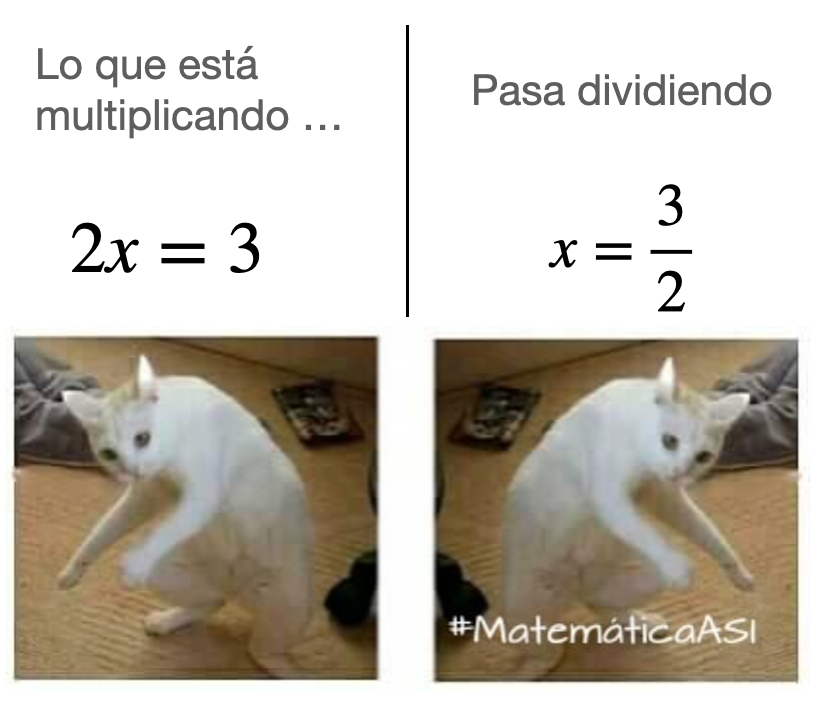
\includegraphics[width=0.4\textwidth]{img-ecc/ecc01.png}
\end{figure}
\end{multicols}

\begin{destacado}
Las ecuaciones de primer grado siempre tendrán solución única, o infinitas soluciones o carecerán de solución alguna.
\end{destacado}


\begin{table}[H]
\centering
\begin{tabular}{|cc|}
\hline
\multicolumn{2}{|c|}{\textbf{Soluciones ecuación primer grado: $\quad \boldsymbol{ax=b}$}} \\ \hline
\multicolumn{1}{|c|}{$a \neq 0$} & \begin{tabular}[c]{@{}c@{}}Ecuación determinada.\\ $x=\dfrac b a$ \\ Solución única \end{tabular} \\ \hline
\multicolumn{1}{|c|}{$a=0, \ \ b=0$} & \begin{tabular}[c]{@{}c@{}} Ecuación indeterminada.\\ $0\cdot x=0 \to \forall x \in \mathbb R$ \\ Infinitas soluciones. \end{tabular} \\ \hline
\multicolumn{1}{|c|}{$a=0,\ \ b\neq 0$} & \begin{tabular}[c]{@{}c@{}}Ecuación incompatible.\\ $0\cdot x=b\neq 0 \to \nexists x$ \\  Sin solución. \end{tabular} \\ \hline
\end{tabular}
\end{table}



\begin{miejemplo}

\begin{footnotesize}
$$\dfrac{3x-2}{6}-\dfrac{3[x-3(x-2)]}{4}=x-2\left[ \dfrac{x+2}{3}-3\left( x-\dfrac{x+1}{4} \right) \right]$$


\vspace{5mm} $ QP:\qquad \dfrac{3x-2}{6}-\dfrac{3x-9(x-2)}{4}=x-\dfrac{2(x+2)}{3}+6\left( x-\dfrac{x+1}{4} \right)$

\vspace{2mm} $QP:\qquad \dfrac{3x-2}{6}-\dfrac{-6x+18}{4}=x-\dfrac{2x+4}{3}+6 x-\dfrac{3(x+1)}{2} $

\vspace{2mm} $QD:\qquad 12\cdot \dfrac{3x-2}{6}-12\cdot \dfrac{-6x+18}{4}=12\cdot 7x-12\cdot \dfrac{2x+4}{3}-12\cdot \dfrac{3x+3}{2}\ \ $ \begin{tiny} ${MCM(6,4,3,2)=12}$\end{tiny}

\vspace{2mm} $QD:\qquad 2(3x-2)-3(-6x+18)=84x-4(2x+4)-6(3x+3)$

\vspace{2mm} $QP:\qquad 6x-4+18x-54=84x-8x-16-18x-18$

\vspace{2mm} $AT:\qquad 6x+18x-84x+8x+18x=-16-18+4+54$

\vspace{2mm} $D:\qquad -34x=24 \ \to \ x=-\dfrac{24}{34}=-\dfrac{12}{17}$
\end{footnotesize}	
\end{miejemplo}

%%%%%%%%%%%%%
\begin{myexampleblock}{Epitafio de Diofanto}

\begin{figure}[H]
	\centering
	
\includegraphics[width=1\textwidth]{img-ecc/ecc09.jpeg}
	\caption*{\scriptsize{Exposiciones Eureka: $\ \ $ https://www.facebook.com/Exposiciones-Eureka-484780888274874/}}
\end{figure}
	
\end{myexampleblock}




\vspace{5mm}
\subsection{Ecuaciones de segundo grado}

\begin{tikzpicture}
	\fill [left color=red!50, right color=teal!50] (0,0) rectangle (3.5,.01);
	\fill [left color=teal!50, right color=blue!50] (3.5,0) rectangle (7.5,.01);
	\end{tikzpicture}
\vspace{0.5cm}

\begin{definition}[ Ecuación de segundo grado]
. Una ecuación de segundo grado con una incógnita es una igualdad algebraica que se puede expresar de la forma: $\quad ax2 + bx + c = 0 $                     siendo $a$, $b$ y $c$ números reales y  $a \neq 0$.
\end{definition}


Si  $b$ y $c$  son números distintos de cero, se dice que la ecuación es completa. Se resuelve por el método general.

Si  $b = 0  \ \vee \   c = 0$ , la ecuación se denomina incompleta. Aunque se pueden resolver por el método general es más sencillo sacar factor común o despejar (ver ejemplo siguiente).


\begin{theorem}[ Resolución de la ecuación de segundo grado. Método general]

$$ax^2+bx+c=0\, , \ a\neq 0 \qquad \Rightarrow \qquad 
\boxed{ \ \boldsymbol{ x\ =\ \dfrac{-b\pm \sqrt{\, b^2\, -\, 4ac \, }}{2a} } \ }$$	
\end{theorem}

\underline{Demostración}: se basa en completar un cuadrado.

$ax^2+bx+c=0 \to a\left(x^2+\dfrac b a x+\dfrac c a \right)=0\, , \  $ como $a\neq 0 \to$

$\to x^2+\dfrac b a x+\dfrac c a=0 \ \to \underbrace{\left( x+\dfrac{b}{2a} \right)^2 }_{x^2+2x\dfrac{b}{2a}+\dfrac{b^2}{4a^2}}-\dfrac{b^2}{4a^2}+\dfrac c a = 0 \to \left( x+\dfrac {b}{2a} \right)^2 = \dfrac{b^2}{4a^2}-\dfrac{c}{a} = \dfrac{b^2-4ac}{4a^2}$ 

Sacando raíz cuadrada: $\ \ \left| x+\dfrac {b}{2a}\right|=\sqrt{ \dfrac{b^2-4ac}{4a^2} } \ \to \ x+\dfrac {b}{2a}=\pm \dfrac{\sqrt{ b^2-4ac }}{2a} $

Despejando $\ \ x=-\dfrac{b}{2a}\pm \dfrac{\sqrt{ b^2-4ac }}{2a}=\dfrac{-b\pm \sqrt{b^2-4ac}}{2a}$ \QED

\vspace{5mm} 

\begin{multicols}{2}
\begin{adjustwidth}{10pt}{40pt}

\begin{destacado}
Las ecuaciones de segundo grado siempre tendrán dos soluciones, una sola (que será doble) o carecerán de ellas (ninguna solución).
\end{destacado}
\end{adjustwidth}

\begin{table}[H]
\centering
\begin{tabular}{|c|c|}
\hline
\begin{tabular}[c]{@{}c@{}}Discriminante\\ $\Delta=b^2-4ac$\end{tabular} & \begin{tabular}[c]{@{}c@{}}Soluciones\\ $ax^2+bx+c=0$\end{tabular} \\ \hline
$\Delta >0$ & 2 soluciones distintas \\ \hline
$\Delta =0$ & 1 solución (doble) \\ \hline
$\Delta<0$ & $\nexists$ solución. \\ \hline
\end{tabular}
\end{table}
\end{multicols}

\begin{multicols}{2}
\underline{Nota}: 

Al resolver una ecuación de segundo grado por la fórmula general es necesario que todos los términos estén agrupados a un lado de la ecuación y ésta igualada a cero.

\begin{figure}[H]
	\centering
	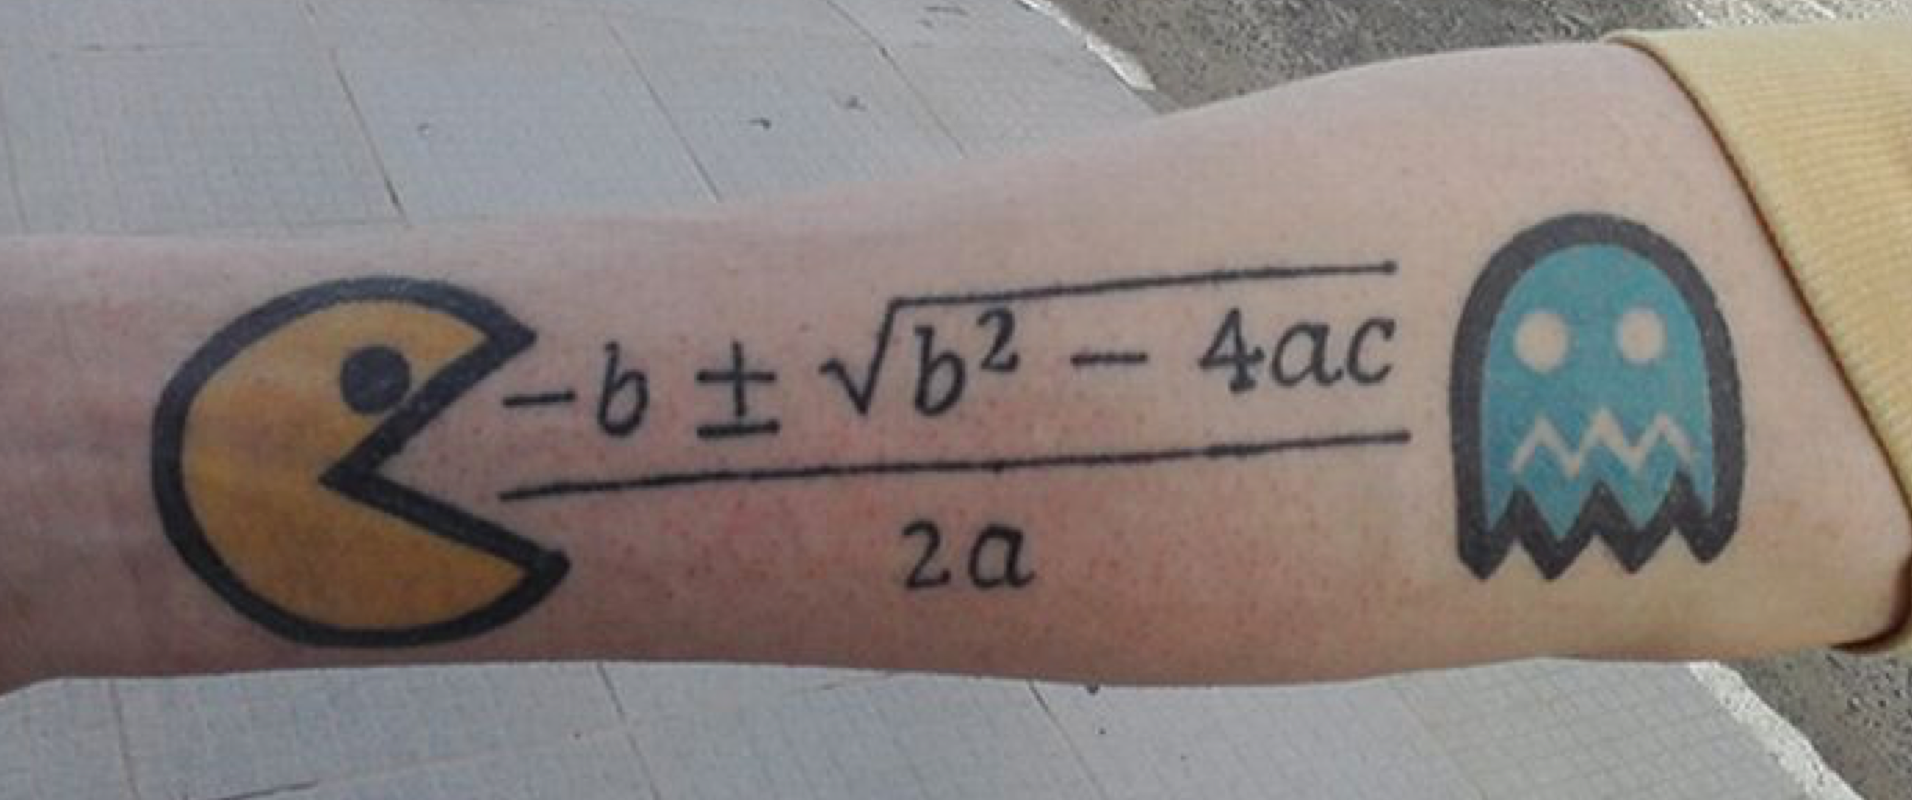
\includegraphics[width=.45\textwidth]{img-ecc/ecc07.png}
\end{figure}
\end{multicols}

\begin{miejemplo}
. Resuelve las ecuaciones: $\qquad  a)\ 6x^2+7x-20=0;\quad b)\ 2x^2+3x=0;\quad c)\ 4x^2-25$ 	

\vspace{5mm} $\triangleright \ \ a)\ \ 6x^2+7x-20=0 \to x=\dfrac{-7\pm \sqrt{7^2-4\cdot 6\cdot (-20)}}{2\cdot 6}=\dfrac{-7\pm \sqrt{49+480}}{12}=\dfrac{-7\pm 23}{12}\to \ x=4/3 \, \vee \, x=-5/2$

\vspace{5mm} $\triangleright \ \ b)\ \ 2x^2+3x=0 \ \ $ Es una ecuación de segundo grado incompleta en la que se puede sacar \emph{factor común} (se puede resolver por el método general con $a=2,\, b=3,\, c=0$):

$2x^2+3x=x\cdot(2x+3)=0 \to \begin{cases} \ \qquad \qquad x=0 & \text{una solución} \\ 2x+3=0 \to x=-3/2 & \text{otra solución} \end{cases}$


\vspace{5mm} $\triangleright \ \ c)\ \ 4x^2-25\ \ $  Es una ecuación de segundo grado incompleta en la que se puede \emph{despejar} (se puede resolver por el método general con $a=4,\, b=0,\, c=-25$):

$4x^2-25=0 \to 4x^2=25 \to x^2=\dfrac{25}{4} \ $ Sacando raíz cuadrada: $|x|=\dfrac 5 2 \to \begin{cases} \  x=\ \ 5/2  \\ \ x=-5/2\end{cases}$
\end{miejemplo}

\begin{miejercicio}

Resuelve las ecuaciones: $\qquad  a)\ x^2-2x+3=0;\qquad b)\ x^2-4x+4=0;\qquad c)\ 3x^2+27=0$

\rule{250pt}{0.1pt}

\vspace{2mm} $\triangleright \ \ a) \quad x=\dfrac{2\pm \sqrt{(-2)^2-4\cdot 1\cdot 3}}{2\cdot 1}=\dfrac{-2\pm \sqrt{-8}}{2} \ : \  \nexists \, \ $ No hay solución.

\vspace{5mm} $\triangleright \ \ b) \quad x=\dfrac{4\pm\sqrt{4^4-4\cdot 1 \cdot 4}}{2\cdot 1}=\dfrac{-4\pm 0}{2}=-2\ $ Solución doble.

\vspace{5mm} $\triangleright \ \ c)\ \quad  \text{ Incompleta (despejar) } \ 3x^2=-\ 27 \to x^2=-9 \to \ : \ \nexists \ $ No hay solución.	
\end{miejercicio}


\begin{theorem} [ Propiedades de las soluciones de la ecuación de segundo grado]

$\Box \ $ Sean $\ x_1=\dfrac{-b+\sqrt{b^2-4ac}}{2a} \ $ y  $\ x_2=\dfrac{-b-\sqrt{b^2-4ac}}{2a}\ $	las dos soluciones (raíces) de una ecuación de segundo grado $\ ax^2+bx+c=0$

\vspace{2mm} --- Suma de raíces: $\qquad \boldsymbol{ S\ = \ x_1+x_2} \ =\dfrac{-b+\sqrt{b^2-4ac}}{2a}+\dfrac{-b-\sqrt{b^2-4ac}}{2a}=\dfrac
{ -b + \cancel{ \sqrt{b^2-4ac} }  -b- \cancel{ \sqrt{b^2-4ac} } }
{2a}=\dfrac{-2b}{2a}= \ \boldsymbol{ -\dfrac b a}$

\vspace{2mm} --- Producto de raíces: $\qquad \boldsymbol{P\ = \ x_1\cdot x_2}\ = \dfrac{-b+\sqrt{b^2-4ac}}{2a} \cdot \dfrac{-b-\sqrt{b^2-4ac}}{2a} =
\vspace{2mm} \dfrac{-\cancel{b^2}- (\cancel{b^2}-4ac)}{4a^2}= \dfrac{4ac}{4a^2}= \ \boldsymbol{\dfrac c a}$

\vspace{2mm} $ax^2+bc+c=0 \ \to \ x^2+\dfrac b a x+\dfrac c a =0 \ \to \ x^2- \left( - \dfrac b a \right) x + \dfrac c a = 0 \, , \ $
por lo que son equivalentes las expresiones: $\quad  \boxed{ \ \boldsymbol{ ax^2+bx+c=0 \ \leftrightarrow \ a(x^2-Sx+P=0) } \ }\, $, con $S=x_1+x_2$ y $P=x_1\cdot x_2$

\vspace{7mm} $\Box \quad a(x-x_1)(x-x_2)=a(x^2-2(x_1+x_2)+x_1x_2)=a\left( x^2-\left( -\dfrac b a \right) x-\dfrac c a \right) = ax^2+bx+c $ 

\vspace{2mm} Luego, todo trinomio de segundo grado $ax^2+bx+c$ con raíces $x_1,\ x_2$ se puede factorizar como $ \quad \subrayado{ \boxed{ \  \boldsymbol{ax^2+bx+c \ = \ a(x-x_1)(x-x_2)} \ }}$
\end{theorem}


\subsection{Ecuaciones reducibles a segundo grado}

\begin{tikzpicture}
	\fill [left color=red!50, right color=teal!50] (0,0) rectangle (3.5,.01);
	\fill [left color=teal!50, right color=blue!50] (3.5,0) rectangle (7.5,.01);
	\end{tikzpicture}
\vspace{0.5cm}

\begin{definition}[ Ecuaciones reducibles a segundo grado (bicuadradas)]

Son ecuaciones del tipo: $\quad \boldsymbol{ax^{2n}+bx^n+c=0}\, . \ $  El  cambio $\ \boxed{\ \boldsymbol{x^n=t} \ } \ $ convierte la ecuación en una de segundo grado: $\ at^2+bt+c=0\, . \ $ 

\vspace{2mm} Una vez resuelta esta ecuación hay que deshacer el cambio establecido: $\ x=\sqrt[n]{t}$
	
\end{definition}


\begin{miejemplo}

Resuelve $\quad a)\ \ x^6-7x^3-8=0;\qquad b)\ \ x^4-3x^2-4=0;\qquad c) \ \ x^8+17x^4+16=0$	

\vspace{5mm} $\triangleright \quad a)\ \ x^3=t \ \to \ t^2-7t-8=0 \ \to \cdots \to \ \begin{cases}
	\ t=\ \ 8=x^3 & \to \ x=2 \\ \ t=-1=x^3 & \to \ x=-1 \end{cases}$

\vspace{5mm} $\triangleright \quad b)\ \ x^2=t \ \to \ t^2-3t-4=0 \ \to \cdots \to \ \begin{cases}
 \ t=\ \ 4=x^2 	 & \to \ x=2 \, \vee \, x=-2 \\ t=-1=x^2 & \to \ \nexists x
 \end{cases}$

\vspace{5mm} $\triangleright \quad c)\ \ x^4=t \ \to \ t^2+17t+16 = 0 \ \to \cdots \to \ \begin{cases} \ t=\ -1=x^4 & \to \ \nexists x \\ \ t=-16= x^4 &\to \ \nexists x \end{cases}$
\end{miejemplo}

\begin{miejercicio}

Resuelve: $\qquad a)\ \ x^4-4x^2=0;\qquad b)\ \ x^{12}+x^6=0; \qquad c) \ \ x^4-25x^2+144=0$	

\rule{250pt}{0.1pt}

\vspace{2mm} $\triangleright \ \ a)\ \ $ Incompleta, factor común: $\ x^2(x^2-4)=0 \to \begin{cases} \ x^2=0 & \to \ x=0 \\ \ x^2-4=0 & \to \ x=2\, \vee \ x=-2 \end{cases}$

\vspace{2mm} También se hubiera podido resolver con el cambio $\ x^2=t$

\vspace{5mm} $\triangleright \ \ b)\ \ $ Incompleta, factor común: $\ x^6(x^6+1)=0 \to \begin{cases} \ x^6=0 & \to \ x=0  \\ \ x^6+1=0 & \to x=\sqrt[6]{-1}\, \nexists \end{cases}$

\vspace{2mm} También se hubiera podido resolver con el cambio $\ x^6=t$

\vspace{5mm} $\triangleright \ \ c)\ \ x^2=t \to t^2-25t+144 = 0 \to \begin{cases} \ t=\ 4=x^2 & \to \ x=2 \, \vee \, x=-2 \\ t=16=x^2 & \to x=4 \, \vee \, x=-4  \end{cases}$
\end{miejercicio}

\vspace{5mm}

Las ecuaciones reducibles a segundo grado de la forma $ax^4+bx^2+c00$, que se resuelven con el cambio $x^2=t$, reciben el nombre de \textbf{bicuadradas}.



\vspace{0.5cm}
\subsection{Ecuaciones polinómicas}

\begin{tikzpicture}
	\fill [left color=red!50, right color=teal!50] (0,0) rectangle (3.5,.01);
	\fill [left color=teal!50, right color=blue!50] (3.5,0) rectangle (7.5,.01);
	\end{tikzpicture}
\vspace{0.5cm}


\begin{definition}[ Ecuación polinómica]

Una ecuación polinómica es la que está definida a partir de un polinomio.

$$a_0x^n+a_1x^{n-1}+\cdots +a_{n-2}x^2+a_{n-1}x+a_n=0$$	
\end{definition}


\begin{theorem}[ Resolución de ecuaciones polinómicas por factorización]
. Si la ecuación polinómica es de grado igual o superior al tercero y no es reducible a segundo grado, podemos \emph{factorizar} el polinomio y sus raíces serán las soluciones de la ecuación.

\vspace{2mm} Es importante advertir que de este modo solo encontraremos las raíces (soluciones) enteras si probamos por los divisores del término independiente o las soluciones racionales si probamos con divisores del término independiente divididas por divisores del término dominante. Nótese que todo lo dicho hasta el momento será cierto si el polinomio tiene todos sus coeficientes enteros.

\vspace{2mm} El teorema fundamental del álgebra asegura que una ecuación polinómica de grado $n$ tendrá, a lo sumo, $n$ raíces (incluyendo sus órdenes de multiplicidad).
\end{theorem}

\begin{myalertblock}{Imposibilidad de resolver por fórmulas generales las ecuaciones de cualquier grado mayor que 4}
	
	Después de los trabajos exitosos de Cardano, Tartaglia y Ferrari (soluciones a ecuaciones de tercer y cuarto grados), durante siglos muchos matemáticos buscaron de manera infructuosa una fórmula que diera las soluciones de cualquier ecuación de quinto grado. Fue Niels Henrik Abel (1802-1829) quien demostró de manera concluyente que tal fórmula general no existe. Por poco tiempo aún subsistió el problema de decidir para cuáles ecuaciones de grado 5 o superior sí existen tales fórmulas, pero este interrogante fue resuelto de manera final por Evariste Galois (1811-1832). Además de mostrar la \emph{imposibilidad de resolver por fórmulas generales las ecuaciones de cualquier grado mayor que 4}, sus trabajos dieron origen a la Teoría de Grupos.

\begin{flushright}
 Arnold Oostra. Revista Tumbaga (2008), 3, 174-186	
\end{flushright}
\end{myalertblock}


\vspace{5mm}

$a_0x^n+a_1x^{n-1}+\cdots +a_{n-2}x^2+a_{n-1}x+a_0= a_0(x-x_1)^{m_1}\cdot (x-x_2)^{m_2}\cdot \cdots \cdot (x-x_k)^{m_k} = 0 \ \to \ $

Raíces (soluciones) $\qquad \to \ \begin{cases}
\ x-x_1=0 &\to x=x_1 \ \text{ orden m}_1 \\
\ x-x_2=0 &\to x=x_2 \ \text{ orden m}_2 \\
\quad \cdots & \quad \quad \cdots \\
\ x-x_k=0 &\to x=x_k \ \text{ orden m}_k	
 \end{cases}$	


\vspace{2mm} \textcolor{gris}{Nos basamos en la propiedad de que el producto de dos números reales da cero si y solo si alguno de ellos es cero: 
$\quad a \cdot b = 0 \ \leftrightarrow \ a=0 \, \vee \, b=0 \, . \ $ Esto solo ocurre si el producto da cero, para cualquier otro número real hay infinitas posibilidades.}

\begin{miejemplo}

Resuelve: $\qquad x^{6} - 2 \; x^{5} - 18 \; x^{4} + 6 \; x^{3} + 41 \; x^{2} + 8 \; x + 60 = \ 0$	

\vspace{5mm} Ecuación polinómica de orden 6 no reducible a segundo grado $\to$ factorización por Ruffini. Posibles raíces $\pm\{1,2,3,45,6,10,12,15,20,30,60\}$

\begin{multicols}{2}
\begin{table}[H]
\centering
\begin{tabular}{r|rrrrrrr}
 & 1 & -2 & -18 & 6 & 41 & 8 & 60 \\
2 &  & 2 & 0 & -36 & -60 & -38 & -60 \\ \hline
 & 1 & 0 & -18 & -30 & -19 & \multicolumn{1}{r|}{-30} & 0 \\ \cline{8-8} 
-2 &  & -2 & 4 & 28 & 4 & 30 &  \\ \cline{1-7}
 & 1 & -2 & -14 & -2 & \multicolumn{1}{r|}{-15} & 0 &  \\ \cline{7-7}
-3 &  & -3 & 15 & -3 & 15 &  &  \\ \cline{1-6}
 & 1 & -5 & 1 & \multicolumn{1}{r|}{-5} & 0 &  &  \\ \cline{6-6}
5 &  & 5 & 0 & 5 &  &  &  \\ \cline{1-5}
 & 1 & 0 & \multicolumn{1}{r|}{1} & 0 &  &  &  \\ \cline{5-5}
\end{tabular}
\end{table}	

$(x-2)(x+2)(x+3)(x-5)(x^2+1)=0 \leftrightarrow $

%\vspace{2mm} 

$$\begin{cases}
 \ x-2=0 &\to \ x=2 \\	
 \ x+2=0 &\to \ x=-2 \\
 \ x+3=0 &\to \ x=-3 \\
 \ x-5=0 &\to \ x=5 \\
 \ x^2+1=0 &\to \ \nexists x
 \end{cases}$$

\end{multicols}

\end{miejemplo}



\begin{miejercicio}

Resuelve: $\qquad a)\ \ 6x^5+7x^4-9x^3+2x^2=0;\qquad \qquad b)\ \ x^6+x^5-8x^4-8x^3+16x^2+16x=0$

\rule{250pt}{0.1pt}

\vspace{2mm} $\triangleright \quad a) \quad $ Primero, al carecer de término independiente, sacamos factor común. Ahora, el término independiente es $16$ y las posibles raíces $\pm\{1,2,4,8,16\}$. Factorizando el polinomio por Ruffini, como aprendimos el tema anterior:

\vspace{2mm} $6x^5+7x^4-9x^3+2x^2=x^2(x+2)(6x^2+5x+1)=0 \to $

\vspace{2mm} $\qquad \qquad  \to \begin{cases}
 	\ x^2=0  \to \ x=0,\ \text{doble} \\ \ x=-2 \\ 6x^2+5x+1=0 \to \begin{cases}
 	\ x=1/2 \\ \ x=1/3 
 	\end{cases}
 \end{cases}$


\vspace{5mm} $\triangleright \quad b) \quad $ Del mismo modo:

\vspace{2mm} $x^6+x^5-8x^4-8x^3+16x^2+16x=x(x+1)(x-2)^2(x+2)^2=0 \to $

\vspace{2mm} $\qquad \qquad \to \begin{cases}
 	\ x=0 \\ \ (x+1)=0 \to \ x=-1 \\ \ (x-2)^2= 0 \to (x-2)= 0 & \to x=2,\ \text{doble} \\ \ (x+2)^2= 0 \to (x+2)= 0 & \to  x=-2,\ \text{doble}
 \end{cases}$
\end{miejercicio}


\vspace{10mm}
\begin{figure}[H]
	\centering
	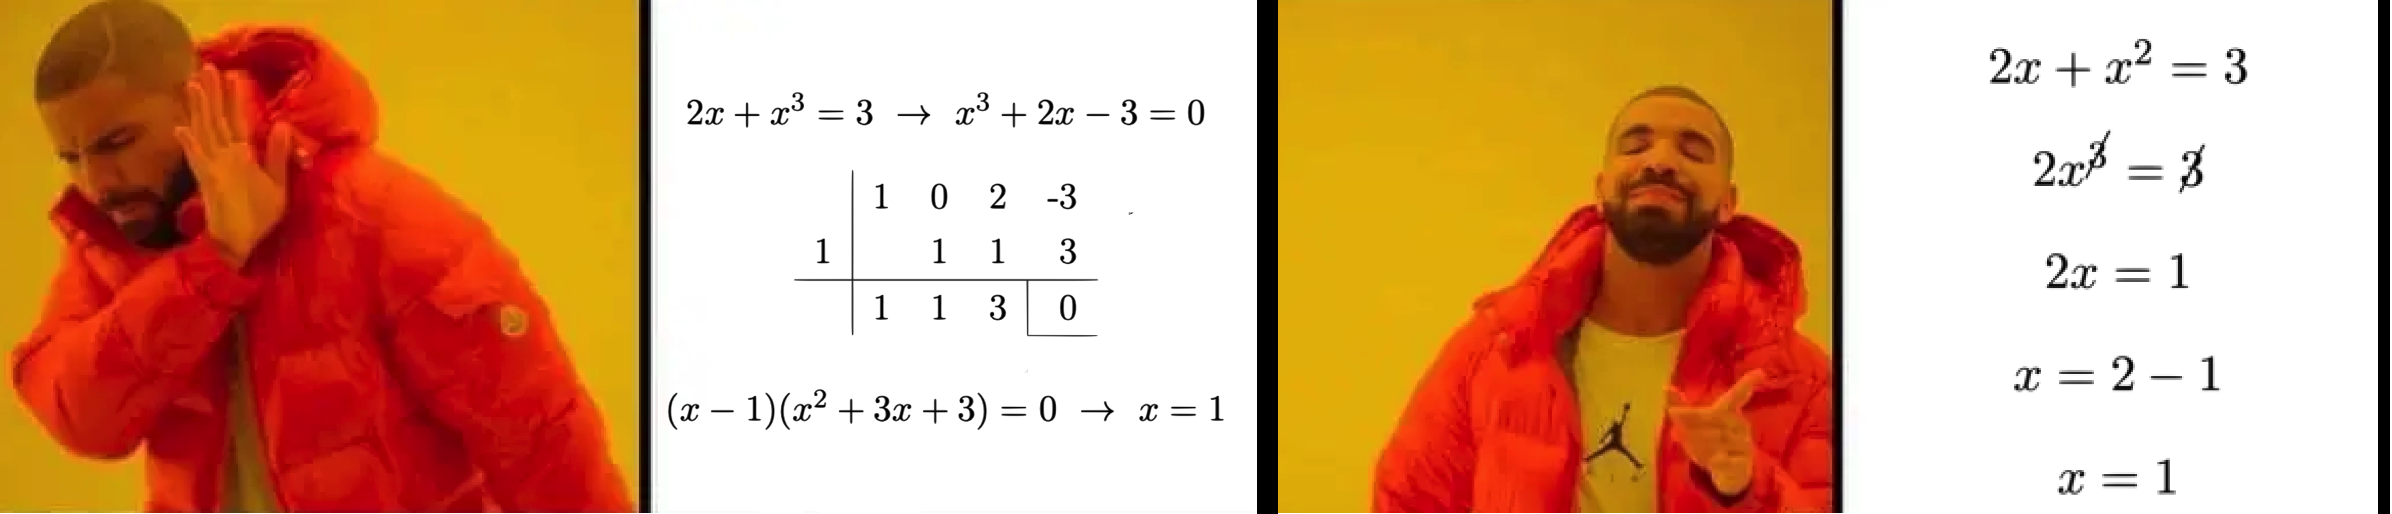
\includegraphics[width=.95\textwidth]{img-ecc/ecc08.png}
\end{figure}

\vspace{1cm}
\section{Ecuaciones racionales}

\begin{tikzpicture}
	\fill [left color=red!50, right color=teal!50] (0,0) rectangle (3.5,.1);
	\fill [left color=teal!50, right color=blue!50] (3.5,0) rectangle (7.5,.1);
	\end{tikzpicture}
\vspace{0.5cm}


\begin{definition}[ Ecuación racional]

Son ecuaciones sobre fracciones algebraicas: $\qquad \dfrac{p(x)}{q(x)}+	\dfrac{r(x)}{s(x)}+\cdots = 0$
\end{definition}



\begin{theorem}[ Resolución de ecuaciones racionales]

Para resolverlas se multiplicará toda la ecuación por el MCM de los denominadores, por lo que tal vez haya que realizar antes algunas operaciones (paréntesis). Con este procedimiento la ecuación racional se convertirá en una ecuación polinómica.


\vspace{5mm} 
\begin{destacado}
\begin{small}
 \textcolor{red}{$\boldsymbol{\boxed{ \ ! \ }} $}  $\ $ \textbf{Resuelta la ecuación hay que comprobar que \emph{las soluciones obtenidas no anulan ningún denominador en la ecuación de partida}.}
 \end{small}
 \end{destacado}
	
\end{theorem}

\begin{miejemplo}

Resuelve: $ \quad \dfrac{x+1}{x-1}-1=\dfrac 1 x$

\vspace{5mm} $MCM:\ \ x(x-1) \ \to \ 	x \cancel{(x-1)} \cdot \dfrac{x+1}{\cancel{(x-1)}}-x(x-1) \cdot 1=\cancel{x} (x-1) \cdot \dfrac 1 {\cancel{x}}$

$x(x+1)=x(x-1)=x-1 \ \to \ x=-1 \ $ Solución (única) que no anula ningún denominador en la ecuación de partida.
\end{miejemplo}

\begin{miejercicio}

Resuelve: $\qquad a)\ \ \dfrac{x+1}{3x-6}-\dfrac{x-1}{2x+4}=\dfrac{10-x^2}{6x^2-24};\qquad b)\ \ 	\dfrac{x}{x+1}-\dfrac{1}{x}=\dfrac{3x+2}{x+1}$

\rule{250pt}{0.1pt}

\vspace{2mm} $\triangleright \quad a)\  $ denominadores:
$3\ x-6=3(x-2);\ \ 2x+4=2(x+2);\ \ 6x^2-24=6(x+2)(x-2) \ \ \to \ \ MCM=6(x+2)(x-2)$

\vspace{2mm} $6(x+2)(x-2) \cdot \dfrac{x+1}{3(x-2)}-6(x+2)(x-2) \cdot \dfrac{x-1}{2(x+2)}=6(x+2)(x-2) \cdot \dfrac{10-x^2}{6(x+2)(x-2)} \to 2(x-2)(x+1)-3(x-2)(x-1)=10-x^2 \ \to \ 15x-12=0 \ \to x=4/5 \ $ Solución (única) que no anula ningún denominador en la ecuación de partida.

\vspace{5mm} $\triangleright \quad b)\ $ Denominadores: $\ MCM=x(x+1)$

\vspace{2mm} $x(x+1)\cdot \dfrac{x}{x+1}-x(x+1)\cdot \dfrac{1}{x}=x(x+1)\cdot \dfrac{3x+2}{x+1} \to \ 2x^2+3x+1=0 \to $

\vspace{2mm} $\to \begin{cases}
 	\ x=-1/2 & \text{ Solución buena, no anula ningún denominador de partida} \\ \ \cancel{\bcancel{ \boldsymbol{ x=-1 }}} & \text{ Solución mala, anula denominadores en la ecc. de partida}
 \end{cases}$

\vspace{2mm} La única solución de esta ecuación es $\ x=-1/2$

\end{miejercicio}


\vspace{1cm}
\section{Ecuaciones irracionales}

\begin{tikzpicture}
	\fill [left color=red!50, right color=teal!50] (0,0) rectangle (3.5,.1);
	\fill [left color=teal!50, right color=blue!50] (3.5,0) rectangle (7.5,.1);
	\end{tikzpicture}
\vspace{0.5cm}


%%%%%%%%%%%%%%%%%%%%%%%%%%
\begin{definition}[ Ecuaciones con raíces cuadradas]

Una ecuación con raíces cuadradas, también llamada ecuación irracional, es aquella en las que la incógnita  aparece bajo el signo de la radical.
\end{definition}

\begin{theorem}[ Resolución de ecuaciones con radicales]


\begin{enumerate}

\item Se aísla el radical en un miembro de la igualdad pasando los restantes términos al otro miembro.


\item Se elevan al cuadrado los dos miembros de la ecuación, con lo que desaparecerá la raíz.


\item Si todavía queda algún radical, se repite el proceso anterior.


\item Se resuelve la ecuación resultante y se \underline{comprueba siempre}$^{(*)}$ cuáles de las soluciones obtenidas verifican la ecuación con radicales de partida.
\end{enumerate}

\vspace{5mm} 
\begin{destacado}
\begin{small}
 \textcolor{red}{$\boldsymbol{\boxed{ \ ! \ }} $}  $\ $ \textbf{Resuelta la ecuación irracional hay que comprobar que \emph{las soluciones obtenidas cumplen la ecuación de partida}.}
 \end{small}
 \end{destacado}

\end{theorem}

$^{(*)}$  Es necesaria siempre la comprobación de las soluciones que se obtengan al resolver este tipo de ecuaciones porque al elevar al cuadrado se pueden introducir soluciones no deseables. P.e.: $\quad x=2 \to x^2=2^2=4 \to \sqrt{x^2}=|x|=2 \ \to x=2 \text{ buena solución; } \cancel{\bcancel{x=-2}} \text{ solución mala}$

\begin{miejemplo}

Resuelve: $\quad x+3\sqrt{x+1}=17$

\vspace{5mm} Paso 1: $\quad x+3\sqrt{x+1}=17 \ \to \ 3\sqrt{x+1}=17-x$

\vspace{2mm} Paso 2: $\quad \left( 3\sqrt{x+1}\right)^2=(17-x)^2 \to 9(x+1)=289-34x+x^2$

\vspace{2mm} No quedan más raíces. No se hace el Paso 3. Resolvemos ahora nuestra ecuación:

\vspace{2mm} Paso 4:  $\quad x^2-43x+280=0 \to \begin{cases} \ x=8 \\ \ x=35 \end{cases}$

\vspace{2mm} Hay que \underline{comprobar} cada una de las soluciones obtenidas en la ecuación de partida. 

\vspace{2mm} $x=8 \to  8+3\sqrt{8+1} = 8+3\cdot 3 = 17 \to \boldsymbol{x=8}\ $ Buena solución.

\vspace{2mm} $x=35 \to  35+3\sqrt{35+1}=35+3\cdot 6=35+18  \ \boldsymbol{\neq} \  17 \to $ Mala solución.

\vspace{2mm} La única solución a nuestra ecuación es: $\quad x=8$.
	
\end{miejemplo}


\begin{miejercicio}

Resuelve las ecuaciones: 

\begin{multicols}{2}
\begin{enumerate}[a) ]
\item $\sqrt{5x+6}=3+2x$
\item $x+\sqrt{7-3x}=1$
\item $\sqrt{3x+4}-\sqrt{1-x}=1$
\item $\sqrt{2x+3}+\sqrt{x-5}=0$	
\end{enumerate}
\end{multicols}

\rule{250pt}{0.1pt}

\vspace{2mm} $\triangleright \ \ a)\ \ \sqrt{5x+6}=3+2x \to \ (\sqrt{5x+6})^2=(3+2x)^2 \to 5x+6=9+12x+4x^2  $

\vspace{2mm} $4x^2+7x+3=0 \to \begin{cases} \ x=-1 \\ \ x=-3/4 \end{cases} \ $ Ahora debemos comprobar los resultados.


\vspace{2mm} $x=-1 \to \sqrt{5(-1)+6} \ ? \  3+2(-1);\ \ 1=3-2 \ $ Sí. Sol. buena.

\vspace{2mm} $x=-3/4 \to \sqrt{5(-3/4)+6}\ ? \ 3+2(-3/4);\ \  \sqrt{-\frac {15}{4} +6} \ ? \ 3-\frac 3 2;\ \ \sqrt{9 4}=\frac 3 2 $ Sí. Sol. buena.

\vspace{2mm} La ecuación tiene dos soluciones válidas, $\ x=-1 \ \wedge \ x=-3/4$

\vspace{5mm} $\triangleright \ \ b)\ \ x+\sqrt{7-3x}=1 \to (\sqrt{7-3x})^2=(1-x)^2 \to 7-3x=1-2x+x^2$

\vspace{2mm} $x^2+x-6=0 \to \begin{cases}\ x=2 \\ \ x=-3 \end{cases}\ $ Ahora debemos comprobar los resultados.

\vspace{2mm} $x=2 \to 2+\sqrt{7-3\cdot 2} \ ? \ 1 \to 2+1 \neq 1 \to $ No. Sol. mala.

\vspace{2mm} $x=-3 \to -3+\sqrt{7-3(-3)}\ ? \ 1 \to -3+4=1\ $ Sí. Sol. buena.

\vspace{2mm} La única solución de la ecuación es $\ x=-3$


\vspace{5mm} $\triangleright \ \ c)\ \ \sqrt{3x+4}-\sqrt{1-x}=1$

\vspace{2mm} Tenemos dos raíces cuadradas. No podemos dejar una sola raíz en un término de la ecuación, al elevar al cuadrado aparecerá una nueva raíz.

\vspace{2mm} $(*) \quad (\sqrt{3x+4}-\sqrt{1-x})^2=1^2 \to (3x+4) -2 \sqrt{3x+4}\cdot \sqrt{1-x} + (1-x)=1$ 

\vspace{2mm} Aislamos la nueva raíz $\ 2x+4=2\sqrt{(3x+4)(1-x)}\ $ y elevamos al cuadrado.

\vspace{2mm} $ (2x+4)^2=(2\sqrt{(3x+4)(1-x)})\  \to  \ 4x^2+16x+16=4\,(3x+4)(1-x)$

\vspace{2mm} $4x^2+16x+16=-12x^2-4x+16 \ \to \ 16x^2+20x=0=x(16x+20) \to  \begin{cases} \ x=0 \\ x=-5/4 \end{cases}$

\vspace{2mm} Hubiese sido mejor dejar una raíz en cada miembro de la ecuación, la raíz que no quede aislada, al elevar al cuadrado volverá a producir una raíz pero más sencilla que anteriormente.

\vspace{2mm} $(**) \quad (\sqrt{3x+4}=(1+\sqrt{1-x})^2\ \to \ (3x+4)=1+2\sqrt{1-x}+(1-x) \ \to \ 4x+2=2\sqrt{1-x}$

\vspace{2mm} $(4x+2)^2=(2\sqrt{1-x})^2 \ \to \ 16x^2+16x+4=4(1-x)  \to \ 16x^2+20x=0=x(16x+20) \to  $

\vspace{2mm} $\to \begin{cases} \ x=0 \\ x=-5/4 \end{cases}\ $ Son más sencillos los cálculos en este caso (una raíz en cada miembro, una de ellas aislada). Por $(*) \  \text{ o por } (**) \ $ tenemos, del mismo modo, que  $x=0\ \wedge \ x=-5/4$. Hay que comprobar las soluciones.

\vspace{2mm} $x=0 \to \sqrt{3\cdot 0+4}-\sqrt{1-0}\ ? \ 1 \to 2-1=1\ $ Sí. Buena solución.

\vspace{2mm} $x=-5/4 \ \to \ \sqrt{3(-5/4)+4}-\sqrt{1-(-5/4)} \ ? \ 1 \ \to \ \sqrt{-\frac {15}{4}+1}-\sqrt{1+\frac 5 4}\ ? \ 1 \ \to \ \sqrt{\frac 1 4}-\sqrt{\frac 9 4 } \ ? \ 1 \ \to \ \frac 1 2 - \frac 3 2 \neq 1 \ $ No. Mala solución.

\vspace{2mm} \normalsize{La} ecuación tiene una sola solución, $x=0$.

\vspace{5mm} $\triangleright \ \ d)\ \ \sqrt{2x+3}+\sqrt{x-5}=0$
	
\vspace{2mm} En esta ocasión, al ser cero el segundo término, es mucho más sencillo aún disponer una raíz en cada término. Sl elevar al cuadrado ambos términos desaparecerán ambas raíces.

\vspace{2mm} $\sqrt{2x+3}+\sqrt{x-5}=0 \to \ (\sqrt{2x+3})^2=(-\sqrt{x-5})^2 \to 2x+3=x-5 \to x=-8$

\vspace{2mm} Hay que comprobar la solución: $\ \ \sqrt{2(-8)+3}+\sqrt{(-8)-5}=0 \to \nexists \sqrt{-13} \ $ por lo que la solución No es válida. Solución mala.

\vspace{2mm} Esta ecuación no tiene soluciones.
	
\end{miejercicio}


\vspace{1cm}
\section{Ecuaciones exponenciales}

\begin{tikzpicture}
	\fill [left color=red!50, right color=teal!50] (0,0) rectangle (3.5,.1);
	\fill [left color=teal!50, right color=blue!50] (3.5,0) rectangle (7.5,.1);
	\end{tikzpicture}
\vspace{0.5cm}


\begin{definition}[ Ecuación exponencial]
. Una ecuación exponencial es aquella en la que la incógnita aparece en el exponente.

$$a^x>0,\ \forall x \in \mathbb R;\qquad x^a=x^b \Rightarrow a=b,\	 \forall a,b \in \mathbb R,\ x\in \mathbb R^+ \smallsetminus \{1\}$$
\end{definition}

\begin{theorem}[ Resolución ecuaciones exponenciales]
. Resolveremos ecuaciones exponenciales: 
\begin{itemize}
\item Expresando, si es posible, ambos miembros de la ecuación como potencias de la misma base e igualando los exponentes.
\item Tomando logaritmos en ambos miembros de la ecuación.
\item Efectuando un cambio de variable $(a^x=t)$. Al final hay que recordar deshacer el cambio de variable establecido.	
\end{itemize}
\end{theorem}

\begin{miejemplo}

$\triangleright \quad \boldsymbol{3^{x-1}=\dfrac 1{27}} \ \to \ 3^{x-1}=\dfrac 1{3^3}\ \to \ 3^{x-1}=3^{-3}\ \Rightarrow \ x-1=-3 \ \to \ \boldsymbol{x=-2}$

\vspace{2mm} Ambos miembros se pueden escribir como una potencia de 3.

\vspace{4mm} $\triangleright \quad \boldsymbol{3^{x-1}=8} \ \Rightarrow \ \ln 3^{x-1}=\ln 8 \ \to \ (x-1)\ln 3= \ln 8 \ \to \ x-1=\dfrac{ln8}{ln3} \ \to \  \boldsymbol{x=1+\dfrac{ln8}{ln3}}$

\vspace{2mm} Un miembro es una potencia de 3 y el otro no. Tomamos logaritmos naturales a ambos lados de la ecuación.

\vspace{4mm} $\triangleright \quad \boldsymbol{3^{x-1}+3^x=4} \ \Rightarrow \ \text{Cambio de variable: } \ \boldsymbol{3^x=t};\ \ 3^{x-1}=\dfrac{3^x}{3}=\dfrac t 3 \ \ \to \ \dfrac t 3 + t=4 \ \to $

$\to \ 4t=12 \ \to \  t=3=3^x \ \Rightarrow \ 3^x=3 \textcolor{gris}{=3^1} \ \to \ \boldsymbol{x=1}$

\vspace{2mm} Aparecen sumas de potencias en un miembro.	Hacemos un cambio de variables, que luego hay que deshacer.
\end{miejemplo}

\begin{miejercicio}

Resuelve: 
\begin{multicols}{2}
  \begin{enumerate}[a) ]
	\item $7^{x-1}=2^{x+5}$

	\item $3^{x-1}+3^x+3^{x+1}=117$

	\item $5^{2x}-30\cdot 5^x+125=0$ 	

	\item $3\cdot 4^{x+1}+2\cdot 2^{x+3}=11$
  \end{enumerate}
\end{multicols}

\rule{250pt}{0.1pt}

\vspace{2mm} $\triangleright \ \ a)\quad 7^{x-1}=2^{x+5}$

\vspace{2mm} Tenemos dos potencias igualadas de distinta base, tomaremos logaritmos (decimales, en este caso, para variar.)

\vspace{2mm} $\mathrm{Log} \, 7^{x-1}=\mathrm{Log} \, 2^{x+5} \ \to \ (x-1) \mathrm{Log} \, 7 = (x+5) \mathrm{Log} \, 2 \ \to \ $

\vspace{2mm}$\to \ x\mathrm{Log}\, 7 -x\mathrm{Log}\, 2=5\mathrm{Log} \, 2+\mathrm{Log}\,7 \to  x(\mathrm{Log}\, 7 -\mathrm{Log}\, 2)=5\mathrm{Log} \, 2+\mathrm{Log}\,7 \ \to \ $
 
\vspace{2mm} $\to \ \boldsymbol{x=\dfrac{5\mathrm{Log} \, 2+\mathrm{Log}\,7}{\mathrm{Log}\, 7 -\mathrm{Log}\, 2}}$



\vspace{5mm} $\triangleright \ \ b)\quad 3^{x-1}+3^x+3^{x+1}=117$

\vspace{2mm} Aparecen sumas de varias potencias, estableceremos un cambio de base: llamamos $\boldsymbol{3^x=t}$, por lo que $3^{x-1}=\frac {3^x}3=\frac t 3;\ 3^{x+1}=3^x\cdot 3=3t$

\vspace{2mm} $\dfrac t 3 +t+3t=117 \ \to \ t+3t+9t=3\cdot 117 \ \to 13t=351 \ \to \ t=\dfrac{351}{13}=27\ = 3^x$

\vspace{2mm} Ahora hay que deshacer el cambio de variable: $3^x=27=3^3 \ \to \ \boldsymbol{x=3}$

\vspace{5mm} $\triangleright \ \ c)\quad 5^{2x}-30\cdot 5^x+125=0$

\vspace{2mm} Aparecen sumas de varias potencias, estableceremos un cambio de base: llamamos  $\boldsymbol{5^x=t}\ \to \ 5^{2x}=(5^x)^2=t^2$

\vspace{2mm} $t^2-30t+125=0 \to \text{ (ec. 2o grado) }\begin{cases}  \ t=25 \\ \ t=5 \end{cases}$

\vspace{2mm} Ahora deshacemos en cambio de variable: $\ \ \begin{cases} \ t=25=5^x & \to \boldsymbol{x=2} \\ \ t=5 =5^x &\to \boldsymbol{x=1} \end{cases}$ 

\vspace{5mm} $\triangleright \ \ d)\quad 3\cdot 4^{x+1}+2\cdot 2^{x+3}=11$

\vspace{2mm} Aparecen sumas de varias potencias, estableceremos un cambio de base: llamamos $\boldsymbol{2^x=t}$, entonces, $\begin{cases} \ 2^{x+3}=2^x\cdot 2^3=8t \\ \ 4^{x+1}=4^x\cdot 4=4\cdot(2^2)^x=4\cdot (2^x)^2=4t^2 \end{cases}$, por lo que

\vspace{2mm} $3(4t^2)+2(8t)=11\ \to \ 12t^2+16t-11=0 \to \text{ (ec. 2o grado) }\begin{cases}  \ t=1/2 \\ \ t=-11/6 \end{cases}$


\vspace{2mm} Ahora, deshacer el cambio de variable: $\begin{cases}
\ t=\dfrac 1 2 = 2^{-1}=2^x	 &\to \boldsymbol{x=-1} \\
\ t=-\dfrac{11}{6}=2^x &\to \boldsymbol{\nexists x }, \ (2^x>0,\ \forall x)
\end{cases}$
\end{miejercicio}



\vspace{1cm}
\section{Ecuaciones logarítmicas}

\begin{tikzpicture}
	\fill [left color=red!50, right color=teal!50] (0,0) rectangle (3.5,.1);
	\fill [left color=teal!50, right color=blue!50] (3.5,0) rectangle (7.5,.1);
	\end{tikzpicture}
\vspace{0.5cm}

\begin{definition}[ Ecuación logarítmica]

Una ecuación logarítmica es aquella en la que la incógnita aparece como argumento de un logaritmo.

$$\log_a(A)=\log_a(B) \ \ \Rightarrow \ \ A=B$$
\end{definition}

\begin{theorem}[ Resolución de ecuaciones logarítmicas]
. Usaremos las propiedades de los logaritmos.	

\vspace{5mm} 
\begin{destacado}
\begin{small}
 \textcolor{red}{$\boldsymbol{\boxed{ \ ! \ }} $}  $\ $ \textbf{Resuelta la ecuación logarítmica hay que comprobar que \emph{las soluciones obtenidas proporcionan argumentos de los logaritmos \textbf{positivos} al sustituir en la ecuación inicial}.}
 \end{small}
 \end{destacado}
\end{theorem}


\begin{miejemplo}
	. Resuelve $\qquad \mathrm{log}\, (x-4)+\mathrm{log}\, (x+5)=1$
	
\vspace{5mm} $\mathrm{log}\, [\, (x-4)\cdot (x+5) \, ]=\mathrm{log}\, 10 \to (x-4)(x+5)=10 \to x^2+x-30=0$

\vspace{2mm} Ecuación segundo grado $\ \to \ x=5 \ \vee \ x=-6$ Hay que comprobar ambas soluciones, que no aparezca ningún argumento no positivo en los logaritmos de la ecuación inicia.

\vspace{2mm} $x=5 \to \begin{cases} x-4=5-4=1>0 \\ x+5=5+5=10>0 \end{cases} \ \boldsymbol{ x=5}\ $ solución buena.

\vspace{2mm} $x=-6 \to \begin{cases} x-4=-6-4=-10<0 \\ x+5=-6+5=-1<0 \end{cases} \ \cancel{\bcancel{\boldsymbol{x=5}}}\ $ solución mala.

\vspace{2mm} Esta ecuación solo tiene una solución, $\ \boldsymbol{x=5}$
\end{miejemplo}

\begin{miejercicio}

Resuelve las siguientes ecuaciones:

\begin{small}
\begin{multicols}{2}
\begin{enumerate}[a) ]
\item $\mathrm{log}\, (x^2-9)-\mathrm{log}\, (x-3)=\mathrm{log}\, 3+\mathrm{log}\, 2x$
\item $3\ln x=\ln 3x+\ln(2x-3)$ 	
\item $\ln 4-\ln(x+2)-\ln(3x-4)+\ln x=0$
\item $2\log_2 x^3=3+\log_2 x$
\item $\log_3 x=\log_9 4$
\item $\log_{x+3}9=\lg_5 3$
\end{enumerate}	
\end{multicols}
\end{small}

\rule{250pt}{0.1pt}

\vspace{5mm} $\triangleright \ \ a) \quad  \mathrm{log}\, (x^2-9)-\mathrm{log}\, (x-3)=\mathrm{log}\, 3+\mathrm{log}\, 2x$

\vspace{2mm} $\log \dfrac{x^2-9}{x-3}=\log 3\cdot 2x \ \to \  \dfrac{x^2-9}{x-3}= \dfrac{(x+3)\cancel{(x-3)}}{\cancel{(x-3)}}=x+3=6x \ \to $

\vspace{2mm} $\to \ 3=5x \ \to \ x=\dfrac 5 3 \ $ Solución buena pues no produce ningún argumento negativo o cero en los logaritmos de la ecuación de partida.


\vspace{5mm} $\triangleright \ \ b) \quad  3\ln x=\ln 3x+\ln(2x-3)$

\vspace{2mm} $\ln x^3=\ln 3x(2x-3) \ \to \ x^3=6x^2-9x \ \to \ x^3-6x^2+9x=0 \ \to \ x(x^2-6x+9)=0 \ \to$

\vspace{2mm} completando cuadrados, $\ \to \  x(x-3)^2=0 \ \to \ \begin{cases}
\ x=0 & \text{ Sol. mala, } \nexists \ln 0 \\
\ x= 3 & \text{ Sol.buena, no } \ln (\le 0)  	
 \end{cases}$

\vspace{5mm} $\triangleright \ \ c) \quad  \ln 4-\ln(x+2)-\ln(3x-4)+\ln x=0$

\vspace{2mm} $  \ln 4-\ln(x+2)=\ln(3x-4)-\ln x \ \to \ \ln \dfrac{4}{x+2}=\ln \dfrac {3x-4}{x}\ \to \ \dfrac{4}{x+2}=\dfrac{3x-4}{x}\ \to$

\vspace{2mm} $\to \ 4x=(x+2)(3x-4) \ \to \ 3x^2-2x-12=0 \ \to \ \begin{cases}
 \ x=2 &  \nexists \ln(\le 0) \text{ buena}  \\ \ x=-4/3 &	\exists \ln(\le 0) \text{ mala}
 \end{cases}$
 
 \vspace{2mm} La única solución de esta ecuación es $x=2$


\vspace{5mm} $\triangleright \ \ d) \quad  2\log_2 x^3=3+3\log_2 x$

\vspace{2mm} Como $3=3\cdot 1=3\, \lg_2 2=\log_2 2^3=\log_2 8$, podemos escribir

\vspace{2mm} $ 2\log_2 x^3=\log_2 8+\log_2 x^3 \ \to \ \log_2 (x^3)^2=\log_2 (8\cdot x^3) \ \to \ \log_2 x^6=\log_2 8x^3 \ \to $

\vspace{2mm}$\to \ x^6-8x^3=0 \ \to \ x^3(x^3-8)=0 \ \to  \ \begin{cases}
 \ x=2 &  \nexists \ln(\le 0) \text{ buena}  \\ 
 \ x=0 &	\exists \ln(\le 0) \text{ mala}	
 \end{cases}$

\vspace{2mm} La única solución de esta ecuación es $x=2$

\vspace{5mm} $\triangleright \ \ e) \quad  \log_3 x=\log_9 4$


\vspace{2mm} Usamos la fórmula del cambio de base de la función logarítmica y lo expresamos todo en función de $\log_3$, por ejemplo.

\vspace{2mm} $\log_3 x=\dfrac{\log_3 4}{\log_3 9}\, ; \ $ como $\log_39=\log_33^2=2\cancelto{1}{\log_3 3}=2\quad \to \quad \log_3 x=\dfrac{\log_3 4}{2} \ \to \ $

\vspace{2mm} $2\log_3 x=\log_3 4 \ \to \ \log_3 x^2=\log_3 4 \ \to \  \ \begin{cases}
 \ x=2 &  \nexists \ln(\le 0) \text{ buena}  \\ 
 \ x=-2 &	\exists \ln(\le 0) \text{ mala}	
 \end{cases}$

\vspace{2mm} La única solución de esta ecuación es $x=2$

\vspace{5mm} $\triangleright \ \ f) \quad  \log_{x+3}9=\lg_5 3$
	
\vspace{2mm} Usamos la fórmula del cambio de base de la función logarítmica y lo expresamos todo en función de $\log_3$

\vspace{2mm} $\dfrac{\log_3 9}{\log_3(x+3)}=\dfrac{\log_3 3}{\log_3 5}\quad  $ Como $log_3 3=1 \ $ y $ \ \log_3 9=\log_3 3^2=2\log_3 3=2\, , \ $

\vspace{2mm} $ \dfrac{2}{\log_3(x+3)}=\dfrac{1}{\log_3 5} \ \to \ \log_3(x+3)=2\log_3 5=\log_3 5^2=\log_3 25 \ \to $

\vspace{2mm} $\to x+3=25 \ \to \ x=22$, solución buena al no hacer que $\nexists \ln(\le 0)$ en ecuación inicial.


\end{miejercicio}

\vspace{1cm}
\section{Ecuaciones con valor absoluto}

\begin{tikzpicture}
	\fill [left color=red!50, right color=teal!50] (0,0) rectangle (3.5,.1);
	\fill [left color=teal!50, right color=blue!50] (3.5,0) rectangle (7.5,.1);
	\end{tikzpicture}
\vspace{0.5cm}

\begin{definition}[ Ecuaciones con valor absoluto]

\begin{theorem}[ Resolución]
. El conjunto de soluciones de una ecuación con valor absoluto viene dado por la siguiente relación:
$\quad |x| = a      \leftrightarrow       x = a    \ \vee \     x = - a\, , \  $
dados $x , a \in \mathbb R  \ \wedge \   a > 0 $
\end{theorem}

\vspace{5mm} 
\begin{destacado}
\begin{small}
 \textcolor{red}{$\boldsymbol{\boxed{ \ ! \ }} $}  $\ $ \textbf{En ecuaciones complicadas (aparece x dentro y fuera del valor absoluto) hay que comprobar \emph{las soluciones obtenidas cumplen la ecuación de partida}. Si estas ecuaciones se resuelven con rigor, estudiando los signos y las zonas de validez, no será necesario.}
 \end{small}
 \end{destacado}
\end{definition}

\begin{miejemplo}
	
	$\left| \dfrac{x+1}{x-5} \right| = 1 \ (\ge 0) \quad \begin{cases}
 \ \dfrac{x+1}{x-5}=1  \ \to \ x+1=x-5 \ \to \ 1=-5 \text{ No puede ser, }  \nexists \text{sol} \\ \\
 \ \dfrac{x+1}{x-5}=-1  \ \to \ x+1=-x+5 \ \to \ 2x=4 \ \to \ x=2 \text{ sol}	
 \end{cases}$
 
\vspace{2mm}  Esta ecuación solo tiene una solución, $\ x=2$
\end{miejemplo}

\begin{miejercicio}

Resuelve la ecuación: $\quad |x+6|=2x+6$

\rule{250pt}{0.1pt}

\vspace{2mm} Primer método, requiere comprobación:

\vspace{2mm} $|x+6|=2x+6 \ \to \ \begin{cases}
\ x+6= \ \ 2x+6 \ \to \ x=0 \\
\ x+6=-(2x+6) \to 3x=-12 \to x=-4	
\end{cases}$


\vspace{2mm} Comprobación: 

\vspace{2mm} $x=0 \ \to |0+6|=|6|=6; \ 2\cdot 0+6=0+6=6\; \ 6=6 \to \text{ Buena (solución válida)}$

\vspace{2mm} $x=-4 \ \to |-4+6|=|2|=2; \ 2\cdot (-4)+6=-8+6=6-2; \ 2\neq -2 \to \text{ Mala (solución no válida)}$

\vspace{2mm} La única solución de esta ecuación es $\ x=0$

\vspace{5mm} Segundo método, con rigor matemático. No hará falta comprobación posterior.

\vspace{2mm} $x+6=0 \leftrightarrow x=-6\ $ Distinguiremos cuando $\ x<6\ $ (que $|x+6|=-(x+6)) \ $ y cuando $\ x\ge 6\ $ (que $|x+16|=x+6$)

% Please add the following required packages to your document preamble:
% \usepackage{multirow}
\begin{table}[H]
\centering
\begin{tabular}{l|c|c|}
\cline{2-3}
 & $]-\infty,-6[$ & $]-6,+\infty[$ \\ \hline
\multicolumn{1}{|l|}{$|x+6|$} & $-x-6$ & $x+6$ \\ \hline
\multicolumn{1}{|l|}{\multirow{4}{*}{$|x+6|=2x+6\quad$}} & $-x-6=2x+6$ & $x+6=2x+6$ \\
\multicolumn{1}{|l|}{} & $3x=12$ & $3x=0$ \\
\multicolumn{1}{|l|}{} & $x=4$ & $\boldsymbol{x=0}$ \\
\multicolumn{1}{|l|}{} & $4 \notin ]-\infty,-6[$ & $0\in [-6,\infty[$ \\ \hline
\end{tabular}
\end{table}

Solución, $\ x=0$	
\end{miejercicio}


\begin{miejercicio}

Resuelve: $\qquad 2|x|+|x-1|=4$

\rule{250pt}{0.1pt}

\vspace{2mm} --- Con rigor:	$\quad x=0;\ \ x-1=0\to x=1$ Diferenciaremos entre $x<0$, $0\le x<1$ y $x\ge 1$, en que cada valor absoluto toma un valor distintos y estudiaremos las distintas posibilidades en una tabla.

% Please add the following required packages to your document preamble:
% \usepackage{multirow}

\begin{table}[H]
\centering
\begin{tabular}{l|c|c|c|}
\cline{2-4}
 & $]-\infty,0[$ & $[0,1[$ & $[1,+\infty[$ \\ \hline
\multicolumn{1}{|l|}{$2|x|$} & -2x & 2x & 2x \\ \hline
\multicolumn{1}{|l|}{$|x-1|$} & -(x-1) & -(x-1) & x-1 \\ \hline
\multicolumn{1}{|l|}{\multirow{4}{*}{$2|x|+|x-1|=4\quad $}} & -2x-(x-1)=4 & 2x-(x-1)=4 & 2x+(x-1)=4 \\
\multicolumn{1}{|l|}{} & -3x=3 & x=3 & 3x=5 \\
\multicolumn{1}{|l|}{} & \textbf{x=-1} & $3\notin [0,1[$ & \textbf{x=5/3} \\
\multicolumn{1}{|l|}{} & $-1\in ]-\infty,0$[ &  & $5/3\in[1,+\infty$[ \\ \hline
\end{tabular}
\end{table}
La ecuación tiene dos soluciones: $\ x=-1 \ \wedge \ x=5/3$

\vspace{5mm} --- Si no lo resolvemos rigurosamente, tendremos que comprobar al  final las soluciones obtenidas. Tendremos que considerar cuatro: $\ |x|=x$, $\ |x|=-x$, para cada uno de ellos, $\ |x-1|=-(x-1)$ y $\ |x-1|=x-1$

\begin{itemize}
\item $2(-x)+[-(x-1)]=4 \ \to \ -3x=3 \to x=-1$	
\item $2(-x)+[(x-1)]=4 \ \ \ \to \ -x=5 \to x=-5$	
\item $2(x)+[-(x-1)]=4 \ \ \ \to \ x=3$	
\item $2(x)+[(x-1)]=4 \ \ \ \ \ \to \ 3x=5 \to x=5/3 $	
\end{itemize}

Comprobaciones:

\vspace{2mm} $x=-1 \to 2|-1|+|-1-1|=2+2=4 \ $ Sí, solución buena.

\vspace{2mm} $x=-5 \to 2|-5|+|-5-1|=10+6\neq 4 \ $ No, solución mala.

\vspace{2mm} $x=3\to 2|3|+|3-1|=6+2\neq 4 \ $ No, solución mala.

\vspace{2mm} $x=5/3 \to 2|5/3|+|5/3-1|=10/3+2/3=4\ $ Sí, solución buena.

\vspace{2mm} La ecuación tiene dos soluciones: $\ x=-1 \ \wedge \ x=5/3$


\end{miejercicio}


\vspace{1cm}
\section{Sistemas de ecuaciones}

\begin{tikzpicture}
	\fill [left color=red!50, right color=teal!50] (0,0) rectangle (3.5,.1);
	\fill [left color=teal!50, right color=blue!50] (3.5,0) rectangle (7.5,.1);
	\end{tikzpicture}
\vspace{0.5cm}

En matemáticas, un sistema de ecuaciones es un conjunto de ecuaciones con más de una incógnita que conforman un problema matemático que consiste en encontrar los valores de las incógnitas que satisfacen todas las ecuaciones del sistema.

Una solución de dicho sistema es un conjunto de valores, uno por cada incógnita, que substituidos en las ecuaciones del sistema hace que éstas se cumplan automáticamente sin que se llegue a ninguna contradicción. 

%\vspace{.5cm}
\subsection{Sistemas de ecuaciones lineales}

\begin{tikzpicture}
	\fill [left color=red!50, right color=teal!50] (0,0) rectangle (3.5,.01);
	\fill [left color=teal!50, right color=blue!50] (3.5,0) rectangle (7.5,.01);
	\end{tikzpicture}
%\vspace{0.5cm}

\begin{definition}[ Sistema lineal de ecuaciones]

Un sistema de ecuaciones lineales (SEL) es un conjunto de dos o más ecuaciones lineales, de primer grado.	
\end{definition}

\begin{theorem} [ Métodos resolución SEL]

\begin{itemize}
\item Sistemas de 2 ecuaciones lineales con 2 incógnitas. Métodos de resolución:
	\begin{itemize}
	\item Igualación: Se elige una de las dos incógnitas y se despejan en ambas ecuaciones, luego se igualan y se encuentra la otra incógnita. Se vuelve a cualquiera de las ecuaciones y se encuentra el valor de la otra incógnita. 
	\item Sustitución: Se elige una ecuación y una de las incógnitas que se despeja y se sustituye su valor en la otra ecuación. Se despeja esta incógnita y, volviendo a cualquier ecuación anterior, se encuentra el valor de la otra incógnita.
	\item Reducción: consiste en combinar ambas ecuaciones (multiplicándolas por los números adecuados) para que al sumarlas desaparezca una de las incógnitas. Se despeja la incógnita que quede y, volviendo a cualquier ecuación anterior, se encuentra el valor de la otra incógnita.
	\end{itemize}
\vspace{5mm}
\item SEL, $m$ ecuaciones con $n$ incógnitas. \emph{Método de Gauss}	: es una generalización del método de reducción. Consiste en encontrar, mediante las transformaciones adecuadas, otro sistema con la mismas soluciones, y en el que cada una de las ecuaciones tiene una incógnita menos que la anterior (sistema escalonado o en cascada).

Se pueden utilizar tres transformaciones ($F_i$, denota a la fila o ecuación que ocupa el lugar $i$.):

\begin{itemize}

\item [---] Cambiar el orden de dos ecuaciones: $\ F_i \leftrightarrow  F_j$


\item [---] Multiplicar los dos miembros de una ecuación por un mismo número distinto de cero: $\ F_i \to t F_i$


\item [---] Cambiar una ecuación por la suma de ella misma más una combinación lineal de otras: $\ F_i \to  F_i + t F_j$
\end{itemize}
\end{itemize}
	
\end{theorem}

\begin{theorem} [ Clasificación de los SEL según el número de soluciones]

Todos los sistemas de ecuaciones lineales pueden tener:

\begin{itemize}
\item [*] Una solución única (para cada una de las incógnitas): se llaman \emph{sistemas compatibles determinados}. $\quad$ \textbf{SCD}
\item [*] Infinitas soluciones: \emph{sistemas compatibles indeterminados}.  $\quad$ \textbf{SCI}
\item [*] No tenr ninguna solución: \emph{sistemas incompatibles}.  $\quad$ \textbf{SI}
\end{itemize}

\end{theorem}

\begin{miejemplo}

Resuelve: $\qquad \begin{cases} \ 2x+5y&=-5 \\ \ 3x-2y&=2 \end{cases}$	

\vspace{5mm} Resolución por \emph{``igualación''}:

\vspace{2mm} Despejamos la $y$ en ambas ecuaciones 

\vspace{2mm} $1^a\ ecc \ \to \  y=\dfrac{-2x-5}{5}\ \ \textcolor{gris}{(1*)};  \qquad\ 2^a\ ecc \ \to \  y=\dfrac{3x-2}{2}\  \ \textcolor{gris}{(2*)}$

\vspace{2mm} Igualando las expresiones obtenidas:  $\ \ \dfrac{-2x-5}{5}\ = \ \dfrac{3x-2}{2} \to $

\vspace{2mm} $\to \ -4x-10=15x-10 \ \to \ \boldsymbol{x=0}$

\vspace{2mm} Podemos sustituir en cualquier ecuación del sistema o en $(1*)$ o en $(2*)$. Yendo a $(1*)$, por ejemplo, $\ \boldsymbol{y=-1}$

\vspace{2mm} Hemos obtenido una solución única (una solución para cada una de las incógnitas), tenemos un \textbf{sistema compatible y determinado, SCD} . Solución: $	\ \boldsymbol{x=0\ \wedge \ y=-1}$

\vspace{7mm} Resolución por \emph{``sustitución''}:

\vspace{2mm} Despejamos la $y$ de la $2^a$ ecuación: $\ y=\dfrac{3x-2}{2}\ \ \textcolor{gris}{(3*)}$

\vspace{2mm} Sustituimos en la otra ecuación, la $1^a$: $\ 2x+5\dfrac{3x-2}{2}=-5$

\vspace{2mm} $4x+5(3x-2)=-10\ \to \ 15=0 \ \to \ \boldsymbol{x=0}$

\vspace{2mm} Sustituyendo el valor encontrado en cualquiera de las ecuaciones del sistema o incluso en $(3*)$, p.e., obtenemos:

\vspace{2mm} $y=\dfrac{3\cdot 0-2}{2} = \dfrac {-2}{2} \ \to \ 	\  \boldsymbol{y=-1}$

\vspace{2mm} Solución:  $\ \ \boldsymbol{x=0\ \wedge \ y=-1} \ \ \textbf{SCD}.$

\vspace{7mm} Resolución por \emph{``reducción''}:

\vspace{2mm} Si lo que deseamos eliminar son las $x$, multiplicaremos la primera ecuación por $3$, la segunda por $(-2)$ y las sumaremos \textcolor{gris}{$(3F_1-2F_2)$}. Si pretendemos eliminar la incógnita $y$, haremos $\ 2F_1+5F_2$, siendo $F_1,\ F_2$ las ecuaciones (filas) $1$ y $2$. Si lo que elegimos es este último caso,

\vspace{2mm} $\begin{cases} \ 2\cdot(2x+5y&=-5)\\ \ 5\cdot(3x-2y&=2) \end{cases} \ \ \to \ \ \begin{cases} \ 4x+10y&=-10 \\ \ 15x-10y&=10 \end{cases} \quad $ Sumando:

\vspace{2mm} $19x=0 \ \to \ \boldsymbol{x=0}$

\vspace{2mm} Sustituyendo, por ejemplo en primera ecuación: $\quad 2\cdot 0 + 5y=-5 \ \to \ \boldsymbol{y=-1}$

\vspace{2mm} Solución:  $\ \ \boldsymbol{x=0\ \wedge \ y=-1} \ \ \textbf{SCD}.$

\end{miejemplo}


\begin{miejercicio}

	Resuelve: $\qquad a)\ \ \begin{cases} \ 3x-2y&=2 \\ \ -6x+4y&=-4 \end{cases} \qquad \qquad  b)\ \ \begin{cases} \ 3x-2y&=2 \\ \  -6x+4y&=0 \end{cases}$	
	
\rule{200pt}{0.1pt}
	
\vspace{2mm}	$\triangleright \ \  a)\ \ \begin{cases} \ 2\cdot (3x-2y=2) \\ \ -6x+4y=-4 \end{cases} \ \to \ \begin{cases} \ 6x-4y&=4 \\ \ -6x+4y&=-4 \end{cases}\ \ $ 

\vspace{2mm} Sumando, $\ 0y=0$, ecuación que se cumple $\forall y \in \mathbb R \ $ En estos casos se suele \emph{parametrizar}: sea $y=\lambda,\ \forall \lambda \in \mathbb R \ \to $ sustituyendo en la primera ecuación del sistema, por ejemplo:

\vspace{2mm} $3x-2\lambda=2 \ \to \ x=\dfrac{2+2\lambda}{3}\, ,\ \forall \lambda \in \mathbb R $

\vspace{2mm} Obtenemos infinitas soluciones, ya que $ \lambda $ puede tomar cualquier valor: tenemos un \emph{sistema compatible indeterminado}, \textbf{SCI:} $\ \boldsymbol {x=\dfrac{2+2\lambda}{3},\ y=\lambda;\ } \ \forall \lambda \in \mathbb R$

\vspace{2mm} Hay infinitas soluciones, por ejemplo, si $\lambda=0 \ \to \ x=2/3,\ y=0$; para $\ \lambda=1 \ \to \  x=4/3,\ y=1$, si $\ \lambda=1/2 \ \to \ x=1,\ y=1/2$, etc.
	
\vspace{7mm}	$\triangleright \ \ b)\ \ \begin{cases} \ 2\cdot(3x-2y=2) \\ \  -6x+4y=0 \end{cases} \ \to \ \begin{cases} \ \ \ 6x-4y&=4 \\ \ -6x+4y&=0 \end{cases}\ \ $

\vspace{2mm} Sumando: $\ 0y=4 \ \to \ $ imposible, no hay ningún número `$y$' tal que al multiplicarlo por $0$ dé $4$, $\ \nexists y \ \to \ \nexists x$

\vspace{2mm} Hemos obtenido un \emph{sistema incompatible}, \textbf{SI}, sin solución.
\end{miejercicio}

\begin{miejemplo}

Resuelve el siguiente sistema de 3 ecuaciones lineales con 3 incógnitas:

\vspace{2mm} $\qquad \begin{cases}
\ x+y+x&=2 \\
\ 2x+3y+5z&=11 \\
\ x-5y+6z&=29	
\end{cases}$	

\vspace{2mm}
\rule{250pt}{0.1pt}

\vspace{4mm}

$\begin{cases}
\ x+y+x&=2 \\
\ 2x+3y+5z&=11 \\
\ x-5y+6z&=29	
\end{cases}\  \Rightarrow \ \mqty[\longrightarrow \\ F_2 \to F_2-2F_1\\ F_3\to
F_3-F_1] \ \Rightarrow \ \left\{
\begin{array}{rcr}
     x+y+x & = & 2 
  \\ y+3z & = & 7
  \\ -6y+5z & = & 27
\end{array}
\right. \ \Rightarrow \ \mqty[ \longrightarrow \\ F_2 \to F_2 \\ F_3\to F_3+6F_2 ] \ \Rightarrow \left\{
\begin{array}{rcr}
     x+y+z & = & 2 
  \\ y+3z & = & 7
  \\ 23z & = & 69
\end{array}
\right. \qquad$ Tenemos un sistema escalonado.

\vspace{2mm} Resolviendo en cascada, de la última ecuación, $\ \boldsymbol{z=}\  \textcolor{gris}{\dfrac{69}{23}}\ \boldsymbol{=3}$

\vspace{2mm} Subiendo un peldaño en la cascada, segunda ecuación, $\textcolor{gris}{y+3\cdot 3=y+9=0 \ \to \  } \ \boldsymbol{y=-2}$

\vspace{2mm} Llegando a la primera ecuación, $\ \textcolor{gris}{x+(-2)+(3)=2 \ \to \ x+1=2 \ \to } \ \boldsymbol{x=1}$

\vspace{2mm} Solución: $\ $ \textbf{SCD} $\ \ \boldsymbol{ x=1 \ \ \textcolor{gris}{\wedge} \ \ y=-2 \  \ \textcolor{gris}{\wedge} \ \ z=3 }$
\end{miejemplo}


\begin{miejercicio}

\begin{small}
$a)\ \left\{
\begin{array}{rrrcr}
     x & + 2y & -z & = & 3 
  \\ 2x & + y & +z & = & 0
  \\  x &  -y & -z & = & 0
\end{array}
\right.;\quad 
b)\ \left\{
\begin{array}{rrrcr}
     x & & +z & = & 3 
  \\ 2x& -y& +4z & = & 8
  \\ x& +y &-z & = & 2
\end{array}
\right.;\quad 
c)\ \left\{
\begin{array}{rrrcr}
     x & & +z & = & 3 
  \\ 2x& -y& +4z & = & 8
  \\ x& +y &-z & = & 1
\end{array}
\right.$
\end{small}

\rule{250pt}{0.1pt}

\vspace{5mm} $\triangleright \quad a)\ \left.
\begin{array}{rrrcr}
     x & + 2y & -z & = & 3 
  \\ 2x & + y & +z & = & 0
  \\  x &  -y & -z & = & 0
\end{array}
\right\} \Rightarrow \mqty[\longrightarrow \\ F_2\to F_2-2F_1 \\ F_3\to F_3-F_1 ] \Rightarrow 
\left.
\begin{array}{rrrcr}
   x&+2y&-z&=&3 \\
    &-3y & +3z&=&	-6 \\
    & -3y & & = & -3
\end{array}
\right\}
$

\vspace{2mm} Resolviendo en cascada: $\quad y=1;\ \ z=-1;\ \ x=0\quad SCD$

\vspace{8mm} $\triangleright \quad  b)\ \left.
\begin{array}{rrrcr}
     x & & +z & = & 3 
  \\ 2x& -y& +4z & = & 8
  \\ x& +y &-z & = & 2
\end{array}
\right\}
\Rightarrow
\left.
\mqty[ \longrightarrow \\ F_2\to F_2-2F_1 \\ F_3\to F_3-F_1  ] \Rightarrow 
\begin{array}{rrrcr}
	x&&+z&=&3\\
	&-y&+2z&=&2 \\
	&y&-2z&=&-1	
\end{array}
\right\} \Rightarrow
$

\vspace{2mm} $\Rightarrow
\mqty[\longrightarrow \\ F_2 \to F_2 \\ F_3\to F_3+F_2 ] \Rightarrow
\left.
\begin{array}{rrrcr}
	x&&+z&=&3\\
	&-y&+2z&=&2 \\
	&&0z&=&1
\end{array} \right\}
\Rightarrow 0\cdot z=1 \to \nexists z \to \ SI\, , \ \text{sin solución.}$ 


\vspace{8mm} $\triangleright \quad c)\ \ \left\{
\begin{array}{rrrcr}
     x & & +z & = & 3 
  \\ 2x& -y& +4z & = & 8
  \\ x& +y &-z & = & 1
\end{array}
\right.
\Rightarrow
\left.
\mqty[ \longrightarrow \\ F_2\to F_2-2F_1 \\ F_3\to F_3-F_1  ] \Rightarrow 
\begin{array}{rrrcr}
	x&&+z&=&3\\
	&-y&+2z&=&2 \\
	&y&-2z&=&-1	
\end{array}
\right\} \Rightarrow$

\vspace{2mm} $\Rightarrow
\mqty[\longrightarrow \\ F_2 \to F_2 \\ F_3\to F_3+F_2 ] \Rightarrow
\left.
\begin{array}{rrrcr}
	x&&+z&=&3\\
	&-y&+2z&=&2 \\
	&&0z&=&0
\end{array} \right\}
\Rightarrow 0\cdot z=0 \to  z=\lambda \in \mathbb R \to $

\vspace{2mm} $ SCI\, , \ \infty \text{ soluciones} \to 2^a \ ecc.\ \ -y+2\lambda=2 \to y=2\lambda - 2 \ \to \ 1^a \ ecc. \ x+\lambda = 3 \to $

\vspace{2mm} $x=3-\lambda\qquad$ Hay infinitas soluciones, $SCI:\ \  x=3-\lambda,\ y=-2+2\lambda,\ z=\lambda;\ \forall \lambda \in \mathbb R$ 

\vspace{2mm} Por ejemplo, si $\lambda=0 \to x=3,y=-2,z=0$. Si $\lambda=1\to x=2,y=0,z=2$, etc.

\end{miejercicio}


\vspace{.5cm}
\subsection{Sistemas de ecuaciones no lineales}

\begin{tikzpicture}
	\fill [left color=red!50, right color=teal!50] (0,0) rectangle (3.5,.01);
	\fill [left color=teal!50, right color=blue!50] (3.5,0) rectangle (7.5,.01);
	\end{tikzpicture}
\vspace{0.5cm}

\begin{definition}[ Sistemas no lineales]

Un sistema de ecuaciones es no lineal cuándo al menos una de sus ecuaciones no es de primer grado.	

\begin{theorem}[ Resolución de sistemas no lineales]

Se pueden usar cualesquiera de los métodos vistos, igualación, sustitución y reducción, el que mejor se adapte en cada caso.	
\end{theorem}

\end{definition}


\begin{miejemplo}

$a)\ \ \left\{ \begin{array}{rcr}
 	2x-y&=&1 \\ x^2-7&=&y+2 
 \end{array} \right.
 \qquad \qquad  b) \left\{
 \begin{array}{rcr}
 x^2+y^2-5x-5y+10&=&0  \\ x^2-y^2-5x+5y+2&=&0
 \end{array} \right.$
 
\vspace{8mm} $\triangleright \ \ a) \quad \left\{ \begin{array}{rcr}
 	2x-y&=&1 \\ x^2-7&=&y+2 
 \end{array} \right.$  
 
\vspace{2mm} Por igualación, despejando `$ y $' en ambas ecuaciones o, por sustitución, despejando `$y$' en la primera ecuación y sustituyendo en la segunda:

\vspace{2mm} $y=2x-1 \ \to \ x^2-7=(2x-1)+2 \to x^2-2x-8=0 \to \begin{cases}\ x=4 \\ \ x=-2 \end{cases} $ 

\vspace{2mm} A valor encontrado para `$x$' le corresponde uno de la `$y$' 

\vspace{2mm} $\ \to \begin{cases}\ x=4  & \to \ y=2\cdot 4-1=7\\ \ x=-2 & \to \  y=2\cdot(-2)-1=-5 \end{cases} $

\vspace{2mm} Esta ecuación tiene \emph{dos parejas} de soluciones: $\ \ x=4 \leftrightarrow y=7 \ \ \wedge \ \ x=-2  \leftrightarrow y=-5$
 
\vspace{8mm} $\triangleright \ \ b) \quad \left\{ \begin{array}{rcr}x^2+y^2-5x-5y+10&=&0  \\ x^2-y^2-5x+5y+2&=&0  \end{array} \right.$
 
\vspace{2mm} Este sistema lo resolveremos por reducción: al sumar ambas ecuaciones desparece la incógnita `$y$'. Y al restarlas, desparece la incógnita `$x$'

\vspace{2mm} Sumando ambas ecuaciones: $\quad 2x^2-10x+12=0  \to \ x^2-5x+6=0 \to \ x=4\ \ \wedge \ \ x=1$

\vspace{2mm} Restando ambas ecuaciones: $\quad 2y^2-10y+8=0  \to \ y^2-5y+4=0 \to \ y=3\ \ \wedge \ \ y=2$

\vspace{2mm} Como, en este caso, las soluciones para $x$ e $y$ no están emparejadas, son independientes entre sí, tenemos 4 parejas de soluciones:

\vspace{2mm} $x=3 \ \wedge \ y=4;\quad x=3 \ \wedge \ y=1;\quad 
x=2 \ \wedge \ y=4;\quad x=2 \ \wedge \ y=1$
 	
\end{miejemplo}

\begin{miejercicio}

Resuelve: $\quad \left\{ \begin{array}{rrr} \dfrac 1 x + \dfrac 1 y &=&1-\dfrac{1}{xy} \\ xy &=& 6 \end{array} \right.$

\rule{250pt}{0.1pt}

\vspace{2mm} Resolveremos el sistema usando la astucia. De la primera ecuación eliminaremos los denominadores multiplicándola por el MCM, `$xy$': $\qquad \quad \left\{ \begin{array}{rrr}  y+x&=&xy-1 \\ xy &=& 6 \end{array} \right.$

\vspace{2mm} Sustituyendo el producto $\ xy=6\ $ en la primera ecuación, $\ \ x+y=5 \quad  \to \ y=5-x \ (*)\ $ 

\vspace{2mm}  De nuevo, llevando este resultado a $\ xy=6\ $, tendremos:
$\ \ x(5-x)=0 \ \to  \begin{cases} \ x=0 \\ \ x=5 \end{cases}$

\vspace{2mm}  Volviendo a la ecuación $\ (*)\ $ obtendremos los correspondientes valores asociados a las $\ y \ $. Tendremos dos parejas de soluciones emparejadas:

\vspace{2mm} $x=0 \ \leftrightarrow \ y=5 \quad \vee \quad x=5 \ \leftrightarrow \ y=0\ $ Soluciones simétricas, ya que las ecuaciones también lo son (se obtiene los mismos resultados si se intercambian los papeles de $x$ e $y$). 

\vspace{2mm} \textbf{Al principio teníamos una ecuación racional, hemos de comprobar que las soluciones obtenidas no anulan ningún denominado como así ocurre efectivamente. Por tanto, las dos parejas de soluciones son válidas.}
	
\end{miejercicio}


%%%
\begin{miejercicio}

Resuelve: $\quad \left\{ \begin{array}{ccc} y\ -\ 2x&=&0 \\ 3^y-6\cdot 3^x&=&-9 \end{array} \right.$

\rule{250pt}{0.1pt}

\vspace{2mm} Por sustitución, de la primera ecuación: $\quad y=2x\ \ (*)$

\vspace{2mm} Sustituyendo en la otra ecuación: $\quad 3^{2x}-6\cdot 3^x=-9$

\vspace{2mm} Se hace necesario un cambio de variable: $\ 3^x=t \ \to 3^{2x}=(3^x)^2=t^2$, luego

\vspace{2mm} $t^2-6t+9=0 \to t=3=3^x \ \Rightarrow \ x=1 \ \to (*):\ \ y=2\cdot 1=2$

\vspace{2mm} Tenemos una única pareja de soluciones. $\quad x=1 \ \leftrightarrow \ y=2$
	
\end{miejercicio}


%%%
\begin{miejercicio}

Resuelve: $\quad \left\{ \begin{array}{ccc} \sqrt{x^2+5}&=&y+2 \\ \log 5x- \log y&=&1\end{array} \right.$

\rule{250pt}{0.1pt}

\vspace{2mm} Trabajamos primero la segunda ecuación: $\ \ \log 5x- \log y=\log \dfrac{5x}{y}=1=\log 10 \ \to \ $

\vspace{2mm} $\to \ \dfrac{5x}{y}=10 \ \to \ 5x=10y \ \to x=2y\ (*)$

\vspace{2mm}  Resultado que sustituimos en la primera ecuación: $\ \sqrt{(2y)^2+5}=y+2 \ \to $

\vspace{2mm} $\to  \ (2y)^2+5=(y+2)^2 \ \to \ 4y^2+5=y^2+4y+4 \ \to \ 3y^2-4y+1=0$

\vspace{2mm} Ecuación que tiene por soluciones $\ y=1 \ \ \wedge \ \ y=1/3$, para cada una de ellas encontraremos su $x$ correspondiente, sin más que sustituir en $(*)$:

\vspace{2mm} Hay dos parejas de soluciones: $\quad y=1 \ \leftrightarrow \ x=2 \quad  \wedge \quad  y=1/3 \ \leftrightarrow \ x=2/3$

\vspace{2mm} \textbf{Venimos de una ecuación irracional y de una logarítmica. Hemos de comprobar la validez o no de las soluciones obtenidas. Ninguno de los cuatro valores de $x$ e $y$ provocan argumentos cero o negativos en los logaritmos. comprobando en la ecuación irracional, $x=2, \ y=1 \ \to \ 3=3\, , \ $ es válida. Para $ x=2/3,\ y=1/3 \ \to \ 7/3=7/3\, , \ $ también válida. Ambas parejas de soluciones son, pues, válidas. }
	
\end{miejercicio}


%%%
\begin{miejercicio}

Resuelve: $\quad \left\{ \begin{array}{ccc} \log(x^2+y)-\log(x-2y)&=&1 \\ 5^{x+1}&=&25^{y+1} \end{array} \right.$

\rule{250pt}{0.1pt}

\vspace{2mm} \begin{small} De la ecuación logarítmica: $\quad \log \dfrac{x^2+y}{x-2y}=\log 10 \ \to \ \dfrac{x^2+y}{x-2y}=10 \ \to x^2+y=10(x-2y)$ \end{small}

\vspace{2mm} Ahora, con la ecuación exponencial: $\quad 5^{x+1}=(5^2)^{y+1}\ \to \ x+1=2(y+1)$

\vspace{2mm}  Nuestro sistema se ha convertido en $\quad \left\{ \begin{array}{rrr} x^2+y&=&10(x-2y) \\ x+1&=&2(y+1) \end{array} \right.$

\vspace{2mm}  De la última ecuación, $x=2y+1 \ (*)$, sustituyendo en $1^a$ ecuación:

\vspace{2mm} $4y^2+1+4y+y=20y+10-20y \ \to \ 4y^2+5y-9=0$ 

\vspace{2mm} Ecuación con dos soluciones para la $y$, volviendo a $(*)$ encontramos las correspondientes para las $x$:

\vspace{2mm} Soluciones: $\qquad x=3 \ \leftrightarrow \ y=1 \quad \wedge \quad x=-7/2 \ \leftrightarrow \ y=-9/4$

\vspace{2mm} \textbf{Tenemos una ecuación logarítmica en nuestro sistema. Comprobamos que ninguna de las parejas de soluciones obtenidas provocan argumentos negativos o cero en nuestros logaritmos, por lo que ambas parejas de soluciones son válidas.}
	
\end{miejercicio}



\vspace{1cm}
\section{Problemas de ecuaciones con enunciados}

\begin{tikzpicture}
	\fill [left color=red!50, right color=teal!50] (0,0) rectangle (3.5,.1);
	\fill [left color=teal!50, right color=blue!50] (3.5,0) rectangle (7.5,.1);
	\end{tikzpicture}
\vspace{0.5cm}


A la hora de resolver un problema que requiera el planteamiento de una ecuación es conveniente:
\begin{itemize}
\item Leer atentamente el enunciado en su totalidad.
\item Determinar nuestra incógnita, lo que nos piden y llamarla x (e y, z, ... , si hay más y se trata de un sistema).
\item Plantear la ecuación (o el sistema) que relaciona algebraicamente los datos del enunciado y la(s) incógnita(s); para ello, suele ser recomendable hacer una tabla –en los problemas de edades–, o un dibujo –en los de tipo geométrico–, o un diagrama –problemas de mezclas–, etc.
\item Resolver la ecuación o el sistema planteados.
\item Interpretar los resultados obtenidos y comprobar que verifican las condiciones del enunciado.
\end{itemize}

Siempre será más sencillo resolver el problema con una ecuación que con un sistema, si ello es posible, aunque en ocasiones el planteamiento con sistema de ecuaciones será más fácil que con una sola ecuación.

\vspace{5mm}
\begin{miejercicio}


Un automóvil sube las cuestas a $54\; km/h$, las baja a $90\; km/h$ y en llano circula a $80\;  km/h$. Para ir de $A$ a $B$ tarda $2$ horas y 30 minutos, y para volver de $B$ a $A$, 2 horas y 45 minutos. ¿Cuál es la longitud de camino llano entre $A$ y $B$ si sabemos que la distancia entre $A$ y $B$ es de $192\;  km$? 

\rule{250pt}{0.1pt}

\begin{figure}[H]
		\centering
		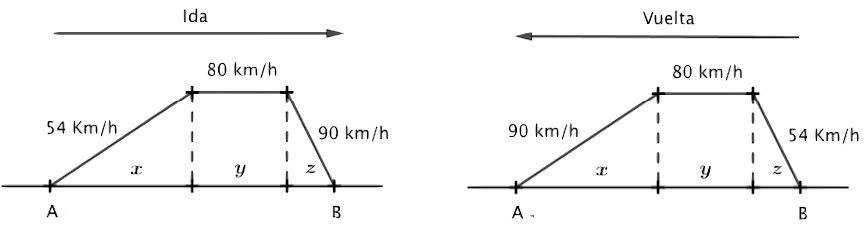
\includegraphics[width=.9\textwidth]{img-ecc/ecc06.png}
\end{figure}

\vspace{2mm} Suponiendo que el vehículo viaja a $v$ constante: $v=\frac s t \to t=\frac s v$. A la ida $t_{ida}=t_{x,s}+t_{y,n}+t_{z,b}$, a la vuelta $t_{vuelta}=t_{x,b}+t_{y,n}+t_{z,s}$, donde los subíndices $\; x,y,z\; $ indican los tramos que circula el coche a distintas velocidades y $\; s,n,b\; $ indican los tramos de `subida', `normal' y `bajada', respectivamente.
	
\vspace{2mm} La traducción del enunciado al leguaje algebraico conduce al sistema:
	
\vspace{2mm} $\begin{cases} x+y+z&=192\\ \frac{x}{54} + \frac{y}{80}+\frac{z}{90}&=2.5 \\ \frac{x}{90}+\frac{y}{80}+\frac{z}{94}&=2.75   \end{cases} \; \; $
	
\vspace{2mm} Lo más cómodo es multiplicar las ecuaciones 2 y 3 por el mcm de los denominadores (2160, en este caso) y conseguir un sistema sin denominadores que, resolviendo por Gauss tiene por solución única (\textbf{SCD}):
	
\vspace{2mm} $\boldsymbol{x=31.725 \; km; \; y= 94.800 \; km; \; z= 65.465 \; km}$, con lo que \textbf{la longitud de camino llano es de} $\boldsymbol{94.8 \; km}$.

\end{miejercicio}

\begin{miejercicio}
. Un tendero invierte 125 \euro $\,$ en la compra de una partida de manzanas. Desecha 20 kg por defectuosas y vende el resto, aumentando 0,40 \euro $\,$ cada kilo sobre el precio de compra, por 147 \euro. ?`Cuántos kilogramos compró?

\rule{250pt}{0.1pt}

\begin{figure}[H]
	\centering
	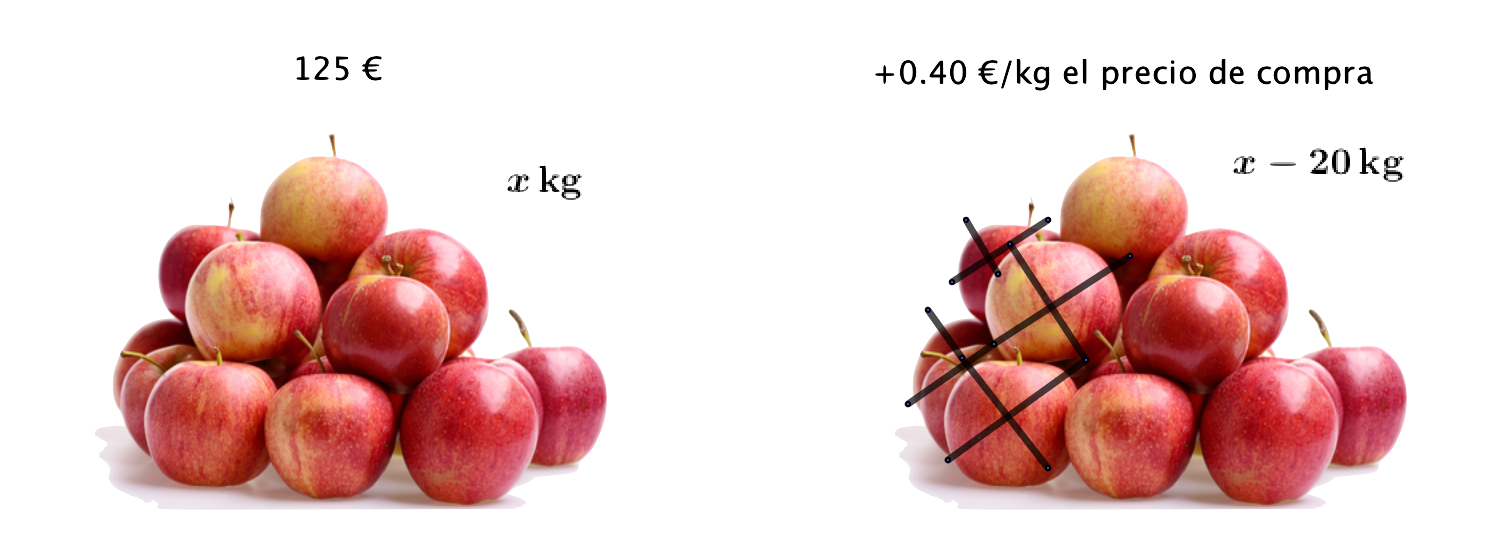
\includegraphics[width=.8\textwidth]{img-ecc/ecc04.png}
\end{figure}
Llamamos $ \ x \ $ a la cantidad de manzanas que compra el tendero inicialmente.

\vspace{2mm} Precio de compra: $\ \dfrac{125}{x}$ \euro/kg, precio de venta: $\ \dfrac{125}{x}+0.40$ \euro/kg. Vendemos un total de $\ x-20$ kg de manzanas. Recaudaremos:

\vspace{2mm} $(x-20)\cdot \left( \dfrac{125}{x}+0.40 \right) = 147 \ \to \ (125+0.4x)(x-20)=147 x \ \to \ 0.4x^2-30x-2500=0$

\vspace{2mm} Soluciones: $ \ x=-50\, , $ no aceptable en el contexto del problema y $\ x=125$, solución que no anula el denominador de nuestra ecuación racional y sí es aceptable.

\vspace{2mm} \textbf{Luego el tendero compra 125 kg de manzanas}.

\vspace{2mm} Comprobación: 125 kg de manzanas le cuestan 125 \euro. Cada kg le ha costado 1 \euro, el precio de compra es de 1 \euro/kg. Si se le estropean 20 kg, le quedan 125-20=105 kg de manzanas que venderá a 1+0.40=1.40 \euro/kg, por lo que recaudará 105$\cdot$1.40$=$147 \euro.

\end{miejercicio}

\begin{miejercicio}
. Dos grifos llenan un depósito de 1500 litros en una hora y doce minutos. Manando por separado, el primero tardaría una hora más que el segundo. ?`Cuánto tardaría en llenar el depósito cada grifo por separado?

\rule{250pt}{0.1pt}

\begin{figure}[H]
	\centering
	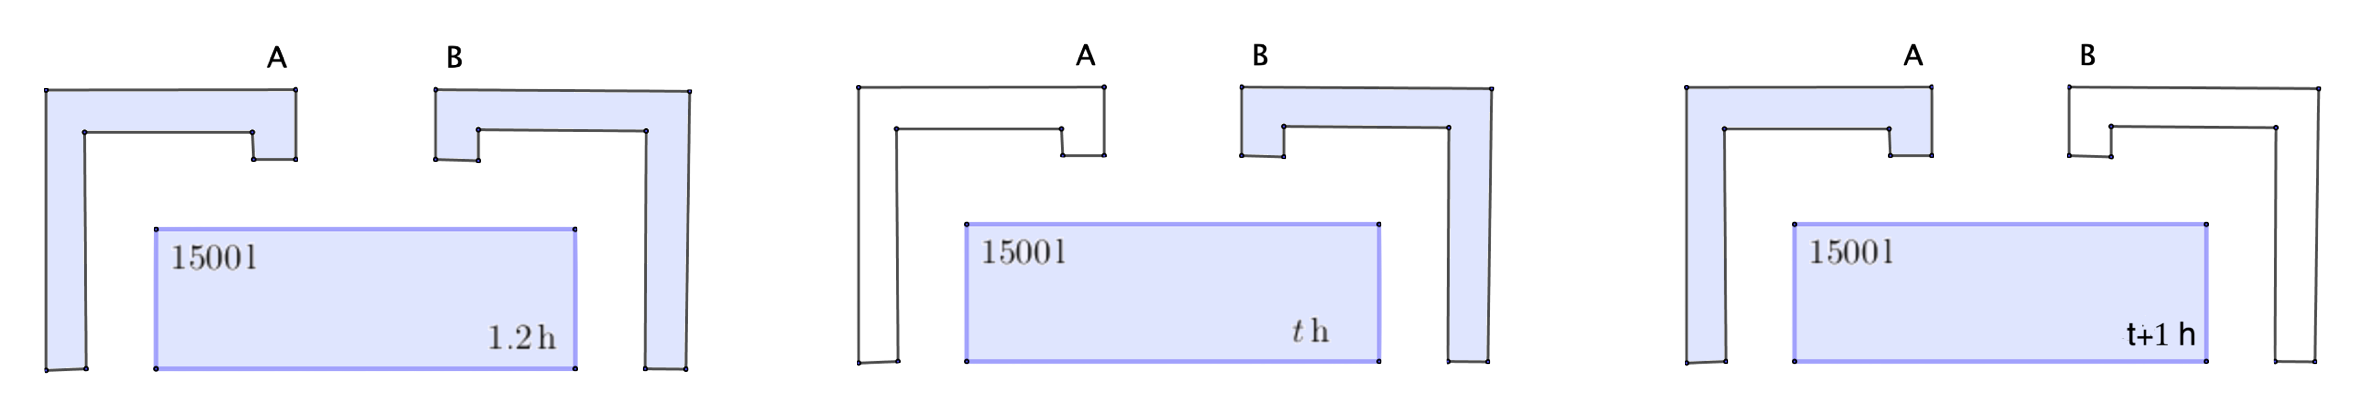
\includegraphics[width=1\textwidth]{img-ecc/ecc03.png}
\end{figure}


Entre los dos grifos vierten 1500 litros en 1.2 horas (1h y 12 min). Como el primero tarda una hora más que el segundo, llamaremos $t$ al tiempo que tardaría el segundo grifo en llenar el depósito con lo que, evidentemente, el primero lo haría en $t+1$ horas.

\vspace{2mm} El primer grifo vierte $\dfrac {1500}{t+1}$ litros cada hora, el segundo $\dfrac {1500} {t} $ l/h. Ambos a la vez vertirán $\dfrac{1500}{1.2}$ l/h. 
$\quad \Rightarrow \quad  \dfrac {1500} {t} +\dfrac {1500}{t+1} = \dfrac{1500}{1,2} \ \to \ \dfrac {1} {t} +\dfrac {1}{t+1} = \dfrac{1}{1,2} \quad MCM:\ 1,2t(t+1)$

\vspace{2mm} $1.2 (t+1) \ + \ 1.2t \ = \ t(t+1) \ \to \ 2.4t+1.2=t^2+t \ \to \ t^2 -1.4 t-1.2=0 \begin{cases} \ t=-0.6\\ \ t=2\end{cases}  $ 

\vspace{2mm} Puesto que la solución de que el grifo B llene el depósito en -0.6 horas (36 min antes de abrirlo)  carece de sentido, la solución es que \textbf{el grifo B tarda 2 horas} en llenar el depósito si está abierto él solo y que \textbf{el grifo A tardará 2+1=3 h} en llenarlo  si solo se abre A.
\end{miejercicio}


%%%%%%%%%%%%%%%%%%%%%%%%%%%%%%%%%%%%%%%%%%%%%%%%%
\vspace{1cm}
\section{Ejercicios}

\begin{tikzpicture}
	\fill [left color=red!50, right color=teal!50] (0,0) rectangle (3.5,.1);
	\fill [left color=teal!50, right color=blue!50] (3.5,0) rectangle (7.5,.1);
	\end{tikzpicture}
\vspace{0.5cm}

%*******
\begin{mipropuesto}
. $a)\ \dfrac{x(x-1)}{2}+\dfrac{(2x-1)^2}{3}=x+1\dfrac x 2; \qquad b) \ \ x(x+4)-5=\dfrac{x(x-1)}{3}$
\end{mipropuesto}
\vspace{-8mm}
\begin{flushright}
	\begin{footnotesize} \textcolor{gris}{\rotatebox{180}{ $a)\ \ x=2 \ \vee \ x=-2/11;\qquad b)\ \ x=1\ \vee \ x=-15/2$ }}	\end{footnotesize}
\end{flushright}

%*******
\begin{mipropuesto}
. $a)\ \ 2x^4-9x^2-5=0;\qquad b)\ \ 	(1-2x^2)^2+3x=2(x+2)^2+2$
\end{mipropuesto}
\vspace{-8mm}
\begin{flushright}
	\begin{footnotesize} \textcolor{gris}{\rotatebox{180}{ $a)\ \ \ x=\pm \sqrt{5};\qquad b)\ \ x=\frac{9\pm \sqrt{153}}{4}$ }}	\end{footnotesize}
\end{flushright}

%*******
\begin{mipropuesto}
. $a)\ \ x^3-4x^2-7x+10=0;\quad b)\ \ x^5+x^4-9x^3-9x^2=0;\quad c)\ \ 6x^4+7x^3+6x^2-1=0$	
\end{mipropuesto}
\vspace{-8mm}
\begin{flushright}
	\begin{footnotesize} \textcolor{gris}{\rotatebox{180}{ $a)\ \ 1,-1,-3/2;\quad b)\ \ 0,1,3,-3;\quad c)\ \ -1/2, -1/3$ }}	\end{footnotesize}
\end{flushright}

%*******
\begin{mipropuesto}
. $a)\ \ \dfrac{48}{5(x-3)}-\dfrac{33}{5(x+2)}+x^2+6=0;\qquad b)\ \ \dfrac{1}{x^2-5x+6}+\dfrac{1}{x^2-4x+3}=\dfrac{1}{x^2-3x+2}$	
\end{mipropuesto}
\vspace{-8mm}
\begin{flushright}
	\begin{footnotesize} \textcolor{gris}{\rotatebox{180}{ $a)\ \ 1,\pm \sqrt{3}; \qquad b)\ \ 0\, ,  \quad MCM=(x-1)(x-2)(x-3)$ }}	\end{footnotesize}
\end{flushright}

%*******
\begin{mipropuesto}
. $a)\ \ 17+\sqrt{169-x^2}=x;\quad b)\ \ \sqrt{2x-1}=\sqrt{3x-2}+\sqrt{1-x};\quad c)\ \ \sqrt{3x+3}-1=\sqrt{8-2x}$	
\end{mipropuesto}
\vspace{-8mm}
\begin{flushright}
	\begin{footnotesize} \textcolor{gris}{\rotatebox{180}{ $a)\ \ \nexists x;\quad b)\ \ x=1;\quad c)\ \ x=2$ }}	\end{footnotesize}
\end{flushright}

%*******
\begin{mipropuesto}
. $a)\ \ \dfrac{4^{x-1}}{2^{x+3}}=17;\qquad b)\ \ 2^{x-1}+2^x+\dfrac{1}{2^x}=\dfrac 7 2;\qquad c)\ \ 8^{x+1}+2^{3x-1}=\dfrac{17}{16}$	
\end{mipropuesto}
\vspace{-8mm}
\begin{flushright}
	\begin{footnotesize} \textcolor{gris}{\rotatebox{180}{ $a)\ \ x=\log_217+5;\quad b)\ \ x=1 \ \vee \ x= -\log_23;\quad c)\ \ x=-1$ }}	\end{footnotesize}
\end{flushright}

%*******
\begin{mipropuesto}
. $a)\ \ \ln(x-3)+\ln(x+1)=\ln 3+ \ln(x-1);\qquad b)\ \ (x-1)\log 3^{x+1}=3\log 3;$

$c)\ \ \log(x^2+3x+36)=1+\log(x+3)$ 	
\end{mipropuesto}
\vspace{-8mm}
\begin{flushright}
	\begin{footnotesize} \textcolor{gris}{\rotatebox{180}{ $a)\ 5;\qquad b)\ 2;\qquad c)\ 1\, , \ 6$ }}	\end{footnotesize}
\end{flushright}

%*******
\begin{mipropuesto}
. $a)\ \ \left| \dfrac{x+2}{5} \right|=x-2;	\qquad \qquad  \qquad  b)\ \ |x^2-x|=|1-x^2|$
\end{mipropuesto}
\vspace{-8mm}
\begin{flushright}
	\begin{footnotesize} \textcolor{gris}{\rotatebox{180}{ $a)\ 4/3;\qquad b)\ 1,\ -1/2$ }}	\end{footnotesize}
\end{flushright}

%*******
\begin{mipropuesto}
. $a)\ \ \begin{cases}	\ \dfrac 3 x - \dfrac x y &=0\\ \ 2x-y&=3 \end{cases};\qquad  b)\ \ \begin{cases} \ \dfrac{x-2}{3}-\dfrac{y-4}{2}=1  \\ \  \dfrac{2}{x-3}=\dfrac{4}{y-2} \end{cases}; \qquad c)\ \ \begin{cases} \ y+2x=x^2\\\ x+y=6 \end{cases} $
\end{mipropuesto}
\vspace{-8mm}
\begin{flushright}
	\begin{footnotesize} \textcolor{gris}{\rotatebox{180}{ $a)\ \ x=3,\ y=3; \qquad  b)\ \ x=7/2,\ y=3; \qquad c)\ \ x=3,\ y=3 \ \ \wedge \ \ x=-2,\ y=8 $ }}	\end{footnotesize}
\end{flushright}

%*******
\begin{mipropuesto}
. 	$a)\ \ \begin{cases} \ 2x-y=9 \\ \ \sqrt{x+y}+y=x \end{cases} ; \qquad \qquad \qquad b) \ \ \begin{cases}  \ x-2y=1\\ \ \sqrt{x+y}-\sqrt{x-y}=2 \end{cases}$
\end{mipropuesto}
\vspace{-8mm}
\begin{flushright}
	\begin{footnotesize} \textcolor{gris}{\rotatebox{180}{ $a)\ \ x=6,\ y=3;\qquad b)\ \ x=17,\ y=8$ }}	\end{footnotesize}
\end{flushright}

%*******
\begin{mipropuesto}
. $a)\ \begin{cases} \ e^x\, e^y=e^9 \\ \ 2^x/4^y=1/8 \end{cases}; \quad b)\ \begin{cases} \ \log(x^2+y)-\log(x-2y)=1 \\ \ 5^{x+1}=25^{y+1} \end{cases};\quad c)\ \begin{cases} \ x^2-y^2=11\\ \ \log x -\log y=1 \end{cases}$
\end{mipropuesto}
\vspace{-8mm}
\begin{flushright}
	\begin{footnotesize} \textcolor{gris}{\rotatebox{180}{ $a)\ x=5,\ y=4;\quad b)\ x=3,\ y=1;\quad c)\ x=10/3,\ y=1/3$ }}	\end{footnotesize}
\end{flushright}

%*******
\begin{mipropuesto}
. $a)\ \left\{\begin{array}{rrr} x+y-z&=&2\\ 2x-2y+3z&=&1 \\ x+2y-z&=&4 \end{array}	\right. ; \quad
b)\ \left\{ \begin{array}{rrr} x+y+x&=&3 \\ -x+2y+z&=&5 \\ x+4y+3z&=&1 \end{array} \right.; \quad
c)\ \left\{  \begin{array}{rrr} x+y+3z&=&2 \\ 2x+3y+4z&=&1 \\ 2x+y+8z&=&7 \end{array} \right.$
\end{mipropuesto}
\vspace{-8mm}
\begin{flushright}
	\begin{footnotesize} \textcolor{gris}{\rotatebox{180}{ $a) \ SCD: \ x=1, y=2, z=1;\quad b)\ SI;\quad c)\ SCI:\ x=5-5\lambda, y=2\lambda-3, z=\lambda$ }}	\end{footnotesize}
\end{flushright}

%*******
\begin{mipropuesto}
.  Determina los valores de $a$ y $b$ para que $x=2$ e $y=3$ sean solución del sistema: 

$\quad \left\{ \begin{array}{rrrr}  \dfrac 5 2 x&-ay &=&3 \\   -\dfrac 1 3 x &+ ay&=&b	 \end{array} \right.$
\end{mipropuesto}
\vspace{-8mm}
\begin{flushright}
	\begin{footnotesize} \textcolor{gris}{\rotatebox{180}{ $a=8/3,\ b=22/8$ }}	\end{footnotesize}
\end{flushright}


%*******
\begin{mipropuesto}
. Resuelve $\qquad \begin{cases} \ (x+1)\, (y+1) = 9 \\ \ (x+2)\, (y-3)=-4 \end{cases}$
\end{mipropuesto}
\vspace{-8mm}
\begin{flushright}
	\begin{footnotesize} \textcolor{gris}{\rotatebox{180}{ $x=2,\ y=-13$ }}	\end{footnotesize}
\end{flushright}
\vspace{-8mm}
\begin{flushright}
	\begin{scriptsize} \textcolor{gris}{\rotatebox{180}{ Desarrolla en iguala $xy$ en ambas ecuaciones, luego despeja una incóginta y sustituye  en cualquier ecuación.}}	\end{scriptsize}
\end{flushright}


%*******
\begin{mipropuesto}
. Dos trabajadores realizan un trabajo en 12 días si lo hacen conjuntamente. Si lo hacen por separado, uno de ello tarda 10 días más en acabarlo que el otro. ?`Cuántos días necesita cada trabajador para realizar la faena por separado?
\end{mipropuesto}
\vspace{-8mm}
\begin{flushright}
	\begin{footnotesize} \textcolor{gris}{\rotatebox{180}{ 30 y 20 días. }}	\end{footnotesize}
\end{flushright}




%%%%%%%%%%%%%%%%%%%%%%%%%%%%%%%%%%%%%%%%%%%%%%%%%

\newpage

$\qquad$


\begin{adjustwidth}{50pt}{250pt}
\begin{cuadro-naranja}
\textbf{\huge{Problemas $\boldsymbol{+}$}}\normalsize{$\, $}
\end{cuadro-naranja}	
\end{adjustwidth}



\vspace{5mm}
\begin{enumerate}[\textbf{P$\boldsymbol +$} 1. ]
\item	$x^{\sqrt{x}}\ = \ x\, \sqrt{x}$

\vspace{-6mm}
\begin{flushright}
\begin{footnotesize} \textcolor{gris}{\rotatebox{180}{ Escribe el segundo miembro en forma de petencia racional de x e identifica exponentes: $\ x=9/4$ }}	\end{footnotesize}
\end{flushright}

\item	$x+y=4;\quad xy=5 \quad \to \quad \dfrac 1 x + \dfrac 1 y = ?$

\vspace{-6mm}
\begin{flushright}
\begin{footnotesize} \textcolor{gris}{\rotatebox{180}{ 4/5 }}	\end{footnotesize}
\end{flushright}

\item	$	\begin{cases} \ x^2+y^2&=30 \\ \ x+y&= 10 \end{cases} \to \ \ $ Calcula $\ xy$

\vspace{-6mm}
\begin{flushright}
\begin{footnotesize} \textcolor{gris}{\rotatebox{180}{ Cuadrado de un binomio suma. $\ \ xy=35$ }}	\end{footnotesize}
\end{flushright}

\item	Si $x+y=7$ y $x^3+y^3=133$, ?`qué vale $xy$?

\vspace{-6mm}
\begin{flushright}
\begin{scriptsize} \textcolor{gris}{\rotatebox{180}{ $x^3+y^3=(x+y)(x^2-xy+y^2) \ \to \ x^2-xy+y^2$ conocido; $x^2-xy+y^2=x^2+2xy+y^2\ - \ 3xy$. Sol. $xy=25$ }}	\end{scriptsize}
\end{flushright}


\item	En un instituto de 300 estudiantes, cada estudiante lee 5 periódicos y cada periódico es leído por 60 estudiantes. ?`Cuántos periódicos hay?

\vspace{-6mm}
\begin{flushright}
\begin{footnotesize} \textcolor{gris}{\rotatebox{180}{ Es importante el número de lecturas. Llama $n=$ al número de periódicos en el centro. $\ n=25$ }}	\end{footnotesize}
\end{flushright}

\item	Una madre es 21 años mayor que su hijo y entro de 6 años la edad de la madre quintuplicará la del hijo. ?`Dónde está el padre?

\vspace{-6mm}
\begin{flushright}
\begin{footnotesize} \textcolor{gris}{\rotatebox{180}{ Junto a la madre. \textcolor{gris}{(hijo=-3/4 año =-9 meses)} }}	\end{footnotesize}
\end{flushright}

\item	$3\log_8x=\log_4(x+6)\, . \ $ Calcula la suma de todas las soluciones de esta ecuación.

\vspace{-6mm}
\begin{flushright}
\begin{footnotesize} \textcolor{gris}{\rotatebox{180}{ Sol 3 (comprueba qué soluciones son válidas) }}	\end{footnotesize}
\end{flushright}

\item	$\log_{\sqrt{2}}\sqrt{x}+\log_2x+\log_4x^2+\log_8x^3+\log_{16}{x^4}=40$

\vspace{-6mm}
\begin{flushright}
\begin{footnotesize} \textcolor{gris}{\rotatebox{180}{ Escribe todos los logaritmos en la misma base. $\ x=64$ }}	\end{footnotesize}
\end{flushright}

\item $\begin{cases} \ \log_xy+\log_yx=17/4 \\ \ xy=288\sqrt{3} \end{cases}$

\vspace{-4mm}
\begin{flushright}
\begin{footnotesize} \textcolor{gris}{\rotatebox{180}{ $x=144 \leftrightarrow y=2\sqrt{3} \  \vee \  x=2\sqrt{3} \leftrightarrow y=144\quad $ Ecuaciones simétricas $\leftrightarrow$ soluciones simétricas.  }}	\end{footnotesize}
\end{flushright}
\vspace{-6mm}
\begin{flushright}
\begin{footnotesize} \textcolor{gris}{\rotatebox{180}{ Trabaja la primera ecuación, usa solo $\log_x$ y resuelve (puedes necesitar un cambio de variable) }}	\end{footnotesize}
\end{flushright}


\item	$\left| \, 3x-|1-2x| \, \right|=2$

\vspace{-6mm}
\begin{flushright}
\begin{footnotesize} \textcolor{gris}{\rotatebox{180}{ $x=1 \, ; \ \wedge \ x=-1/5$ }}	\end{footnotesize}
\end{flushright}

\item	$\sqrt[3]{4x-1}=x-4$

\vspace{-6mm}
\begin{flushright}
\begin{footnotesize} \textcolor{gris}{\rotatebox{180}{ Eleva al cubo. $\quad x=7$ }}	\end{footnotesize}
\end{flushright}


\item	$abx^2-(a+b)x+1=0$

\vspace{-6mm}
\begin{flushright}
\begin{footnotesize} \textcolor{gris}{\rotatebox{180}{ $x=1/a \ \wedge \ x=1/b$ }}	\end{footnotesize}
\end{flushright}

\item	$(a+b)x^2=a-bx$

\vspace{-6mm}
\begin{flushright}
\begin{footnotesize} \textcolor{gris}{\rotatebox{180}{ $x=-1 \ \wedge \ x=\dfrac{a}{a+b}$  }}	\end{footnotesize}
\end{flushright}

\item	$(x-a)^2+x(x-b)=8b^2-x(2a-b)+a^2$

\vspace{-6mm}
\begin{flushright}
\begin{footnotesize} \textcolor{gris}{\rotatebox{180}{ $x=\pm 2b$ }}	\end{footnotesize}
\end{flushright}


\item	Resuelve: $a)\ \ \dfrac{1}{a^2+\dfrac{1}{a+1}}=a-1\, ; \qquad b)\ \ \sqrt{x+\sqrt{4x+\sqrt{16x+\sqrt{64x+5}}}}-\sqrt{x}=1 $

\vspace{-4mm}
\begin{flushright}
\begin{footnotesize} \textcolor{gris}{\rotatebox{180}{ a) bicuadrada, sol. $x=\pm \sqrt{2}\qquad $ b) aisla y eleva al cuadrado repetidamente, sol $\ \ x=1/16$ }}	\end{footnotesize}
\end{flushright}


\item	El mito de Sísifo

\begin{small} \emph{En la mitología griega, Sísifo fue fundador y rey de Éfira, más tarde conocida como Corinto. Era uno de los siete hijos de Eolo y Enareta, y esposo de Mérope, hija de Atlante. Sísifo era un ejemplo de rey impío, pues es conocido por su castigo: empujar cuesta arriba por una montaña una piedra que, antes de llegar a la cima, volvía a rodar hacia abajo, repitiéndose una y otra vez el frustrante y absurdo proceso. El término ``trabajo de Sísifo'', que se utiliza en la actualidad para describir un trabajo duro que debe hacerse una y otra vez, tiene su origen en el castigo de Sísifo} \end{small}

\begin{multicols}{2}
	\begin{figure}[H]
	\centering
	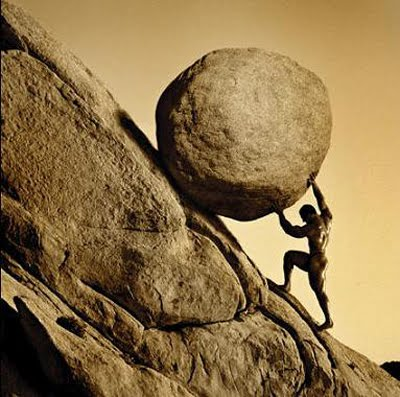
\includegraphics[width=.4\textwidth]{img-ecc/ecc16.jpeg}
\end{figure}

Sísifo debe llevar cada día una piedra a la cima de la montaña. El primer día tarda 7 horas en subir y bajar.

\vspace{2mm} La tarea es pesada y, cada día, tarda el doble que el anterior en subir y la mitad que el anterior en bajar.

\vspace{2mm} Si emplea 8 horas en subir y bajar la piedra el segundo día, ?`cuántas horas tardará en subir y bajar el tercer día?	
	\end{multicols}


\vspace{-6mm}
\begin{flushright}
\begin{footnotesize} \textcolor{gris}{\rotatebox{180}{ El tercer día tarda 13 horas. }}	\end{footnotesize}
\end{flushright}



\end{enumerate}

%%%%%%%%%%%%%%%%%%%%%%%%%%%%%%%%%%%%%%%%%%%%%%%%%
\newpage
\begin{small}
\section{Resumen del tema}

\begin{tikzpicture}
	\fill [left color=red!50, right color=teal!50] (0,0) rectangle (3.5,.1);
	\fill [left color=teal!50, right color=blue!50] (3.5,0) rectangle (7.5,.1);
	\end{tikzpicture}
\vspace{1cm}

\begin{myblock}{Resumen: \emph{``Ecuaciones y sistemas''}}

\vspace{2mm} \textbf{\underline{ECUACIONES}}:

\vspace{4mm} $\triangleright \ \ $ \textbf{Ecuaciones de primer grado}: $\ ax+b = 0   \ \to \ x=-b/a$

\vspace{2mm} Algoritmo:  quitar paréntesis y/o denominadores, trasposición de términos, agrupar y despejar.

\vspace{2mm} Pueden tener 1 solución única, infinitas soluciones o ninguna solución.


\vspace{4mm} $\triangleright \ \ $ \textbf{Ecuaciones de segundo grado}:  $ax^2 + bx + c = 0  \ to \  $ fórmula general  

\vspace{2mm} Ecuaciones incompletas: factor común o despejar

\vspace{4mm} $\triangleright \ \ $ \textbf{Ecuaciones reducibles a 2$^o$ grado} (bicuadradas):  $ax^{2n}+bx^n+c=0  \ \to \ $  el cambio: $x^n=t$ la convierte en una ecuación de segundo grado. Acordarse de deshacer el cambio.

\vspace{4mm} $\triangleright \ \ $ \textbf{Ecuaciones polinómicas}:  (grado mayor o igual a 3) $\to$ Factorizar por Ruffini (esto permite encontrar las soluciones enteras o racionales).

\vspace{4mm} $\triangleright \ \ $ \textbf{Ecuaciones racionales}: (cocientes de polinomios, aparecen x en el denominador). Para eliminar los denominadores hay que multiplicar TODA la ecuación por el MCM de los DENOMINADORES.

\vspace{2mm} \textcolor{red}{$\boldsymbol{\boxed{ \ ! \ }} $}  $\ $ Hay que COMPROBAR SIEMPRE LAS SOLUCIONES obtenidas en la ecuación de partida.

\vspace{4mm} $\triangleright \ \ $ \textbf{Ecuaciones irracionales}: (con la x bajo el símbolo radical): Tendremos que aislar la/las raíz/raices en un miembro de la ecuación y elevar al cuadrado. El proceso puede necesitar de repetición.

\vspace{2mm} \textcolor{red}{$\boldsymbol{\boxed{ \ ! \ }} $}  $\ $ Hay que COMPROBAR SIEMPRE LAS SOLUCIONES obtenidas en la ecuación de partida.

\vspace{4mm} $\triangleright \ \ $ \textbf{Ecuaciones exponenciales}: La incógnita está en el exponente. Podremos usar propiedades de las potencias, logaritmos, a veces será necesario un cambio de variable (acordarse al final de deshacerlo)

\vspace{4mm} $\triangleright \ \ $ \textbf{Ecuaciones logarítmicas}: la x está dentro de algún logaritmo. Usaremos las propiedades de los logaritmos.

\vspace{2mm} \textcolor{red}{$\boldsymbol{\boxed{ \ ! \ }} $}  $\ $ Hay que COMPROBAR SIEMPRE LAS SOLUCIONES obtenidas en la ecuación de partida.

\vspace{4mm} $\triangleright \ \ $ \textbf{Ecuaciones con valor absoluto}: la x aparece dentro del valor absoluto o módulo.$\ $ \textcolor{red}{$\boldsymbol{\boxed{ \ ! \ }} $}  $\ $ Si se resuelven con rigor, estudiando signos, no hay problema. Pero si usamos que $|x|=a\ \leftrightarrow \  x=a  \ \vee \   x=-a$ en expresiones complicadas, habrá que COMPROBAR SIEMPRE LAS SOLUCIONES obtenidas en la ecuación de partida.


\vspace{6mm} \textbf{\underline{SISTEMAS DE ECUACIONES}}:  Sustitución, reducción, igualación. Gauss (SEL).
	
\end{myblock}
\end{small}







\begin{comment}

%%%%%%%%%%%%%%%%%%%%%%%%%%%%%%%%%%%. SECCIONES

PROBLEMAS DE ENUNCIADO *****************************************************

\begin{figure}[H]
	\centering
	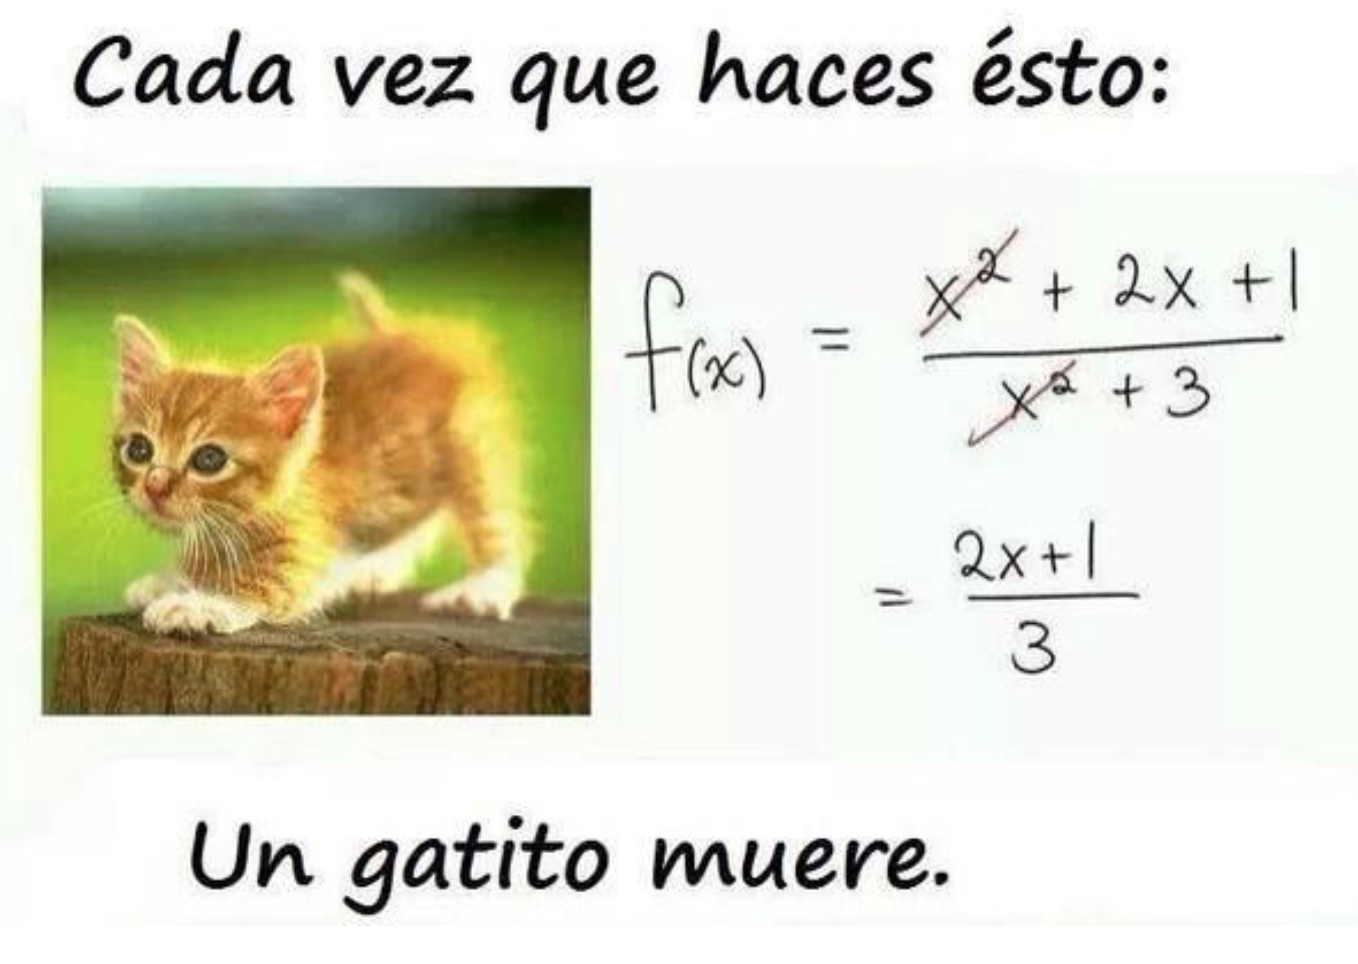
\includegraphics[width=0.35\textwidth]{img-pol/pol05.png}
\end{figure}




\chapter{texto}

\begin{tikzpicture}
	\fill [left color=red!50, right color=teal!50] (0,0) rectangle (6.5,.2);
	\fill [left color=teal!50, right color=blue!50] (6.5,0) rectangle (11.5,.2);
	\end{tikzpicture}

\vspace{1cm}
\section{texto}

\begin{tikzpicture}
	\fill [left color=red!50, right color=teal!50] (0,0) rectangle (3.5,.1);
	\fill [left color=teal!50, right color=blue!50] (3.5,0) rectangle (7.5,.1);
	\end{tikzpicture}
\vspace{0.5cm}

\subsection{texto}

\begin{tikzpicture}
	\fill [left color=red!50, right color=teal!50] (0,0) rectangle (3.5,.01);
	\fill [left color=teal!50, right color=blue!50] (3.5,0) rectangle (7.5,.01);
	\end{tikzpicture}
\vspace{0.5cm}


%%%%%%%%%%%%%%%%%%%%%%%%%%%%%%%%%%%. \begin{ ------>. 
detsacado;  cuadro-naranja;  cuadro-gris;  miejercicio (solución extensa);  mipropuesto (solución corta y fuera del cuadro)

%%%%%%%%%%%%%%%%%%%%%%%%%%%%%%%%%%%. CURIOSIDAD
\vspace{1cm}
\color{ForestGreen!80}
\rule{250pt}{0.2pt}
Texto
\vspace{-8mm}
\begin{flushright}
\rule{250pt}{0.2pt}		
\end{flushright}	
\color{black}
\end{comment}